\chapter{Jet-Hadron Correlations Relative to the Event Plane}
\label{ch:jhcorr}
\begin{itquote}
This chapter is based on \cite{STAR:2023hye} published in \href{https://doi.org/10.1103/PhysRevC.109.044909}{Physical Review C \textcopyright{} American Physical Society}; titled ``Jet-hadron correlations with respect to the event plane in \(\sqrt{s_\mathrm{NN}} = 200\)~GeV Au+Au collisions in STAR''; authored by the STAR Collaboration, with Joel A. Mazer, Tanmay Pani and Sevil Salur as principal authors.
\end{itquote}
As discussed in Sec.~\ref{sec:jetsInQGP}, a parton traversing the QGP loses energy, and the amount lost is expected to depend on the length of its path through the medium.
%
In a non-central collision the overlap region is elongated, so the path length of a jet depends on its direction relative to the event plane (Sec.~\ref{sec:flowIntro} and App.~\ref{sec:EP_Recon}), and this chapter describes the measurement of the distribution of charged hadrons around jets separately for jets at different angles to the event plane.
%
In this analysis, the coordinate system used to depict the distribution of associated particles is defined relative to a reconstructed jet, also called a \emph{trigger jet}. 
%
The distribution is thus given by:
%
\begin{equation}
	\frac{1}{N_{\rm trig}} \frac{d^2 N_{\rm assoc,jet}}{d\dphi d\deta},
	\label{Eq:JHCorrIntro}
\end{equation}
%
\noindent where $N_{\rm trig}$ is the number of trigger jets, $N_{\rm assoc,jet}$ is the number of associated particles, \dphi ($=|\phi_{\rm jet}-\phi_{\rm assoc}|$) is the azimuthal angle of the associated particles relative to the trigger jets, and \deta ($=|\eta_{\rm jet}-\eta_{\rm assoc}|$) is the difference in the pseudorapidities of the trigger jet and associated particle.  
%
When studying the \dphi distributions, a peak is observed at $\dphi = 0$ which is the triggered jet, referred to as the \emph{near-side}.  
%
Another peak which is seen near $\dphi = \pi$ is referred to as the \emph{away-side}.  
%
The away-side consists of the hadrons from the recoiling parton, i.e.\ the second jet of the back-to-back hard scattering.

The goal of this analysis is to study the conditional yield of associated particles, the width of the near- and away-side peaks (quantified using the Gaussian width) as a function of the angle between the jet axis and the event plane.  The yield is estimated by:
%
\begin{equation}
	\mathrm{Yield} = \frac{1}{N_{\rm trig}} \int_{c}^{d} \int_{a}^{b} 
	\frac{d^2N_{\rm assoc,jet}}{d\dphi d\deta}  d\dphi d\deta.
	\label{Eqtn:Yield}
\end{equation}
%
The integration limits are chosen based on practical considerations, including the detector acceptance and binning of histograms.  

\section{Analysis method} \label{sect:Method}
This measurement utilizes data collected during the 2014 run from \AuAu collisions at nucleon-nucleon center-of-mass energy of \sNN{200}{GeV} by the STAR experiment~\cite{ACKERMANN2003624} at RHIC.  Events referred to as signal (same) events are required to fire the high-tower (HT2) trigger of the BEMC~\cite{BEDDO2003725}, which requires a single BEMC tower with a transverse energy above approximately 5.4~GeV.  Minimum-bias (MB) triggered events based on coincidence of Zero Degree Calorimeters (ZDC coincidence), Vertex Position Detectors (VPD) and Beam-Beam Counters (BBC) signals (Sec.~\ref{sec:triggerDetectors}) are used to estimate the pair-acceptance effects via a mixed-event (ME) technique \cite{PhysRevC.96.024905}. For this analysis, 9.4M HT-triggered and 4.0M MB collision events in the 20--50\% centrality range are used.

\subsection{Data set and event selection} \label{sec:JHEventSel}
The data consist of the mid- and low-luminosity subsets of the 2014 \AuAu production (830 and 548 runs, respectively).
%
Runs are rejected when run-averaged quantities of the MB events, namely the mean primary-vertex position along the beam $\langle v_z \rangle$ and in the transverse plane $\langle V_r \rangle$, the ZDC coincidence rate $\langle \mathrm{ZDCx} \rangle$, the reference multiplicity $\langle \mathrm{refMult} \rangle$, and the mean track transverse momentum, lie more than three standard deviations from their average over all runs; such outliers indicate detector or beam conditions that are not representative of the data set.

Events are required to have a reconstructed primary vertex within $|v_{z}| < 24$~cm of the center of the detector.
%
The pseudorapidity acceptance of the TPC changes with the vertex position, and the MB sample used for the event mixing (Sec.~\ref{sect:MixedEvents}) contains very few events at large $|v_z|$, which would limit the precision of the acceptance correction; the value of 24~cm was chosen by balancing the available statistics against the size of the resulting systematic uncertainties.
%
Events containing a track with $\ensuremath{p_{\rm T}}\xspace > 30$~\GeVc are rejected, since such tracks are dominated by cosmic rays and mis-reconstructed tracks for which the TPC momentum resolution is poor.

The centrality of each event, defined in Sec.~\ref{sect:CentEP}, is determined from the charged-particle multiplicity measured in the TPC within $|\eta| < 0.5$ (refMult) using the standard STAR procedure: refMult is corrected event-by-event for its dependence on the vertex position and on the luminosity, and the multiplicity distribution of the most peripheral events is corrected for the trigger inefficiency of the VPD using a Monte Carlo Glauber simulation.
%
The 20--50\% centrality range used here corresponds approximately to corrected refMult values of 75--250.
%
To increase the number of events available for the event mixing by more than 60\%, events from two MB triggers with different online VPD vertex requirements are combined: VPDMB5 and VPDMB30, which require the vertex position reconstructed online from the VPD timing to lie within \(|v_{z}| < 5\)~cm and \(|v_{z}| < 30\)~cm of the center of the detector, respectively.
%
The VPDMB5 events are reweighted in bins of refMult and $v_z$ so that their multiplicity distributions match those of the VPDMB30 events, which compensates for the different VPD resolution and the offset of the online VPD vertex cut, and they are only used for $|v_z| < 16$~cm; events in which both triggers fired are used only once.

\subsection{Track and tower selection} \label{sec:TrackTowerSel}
Charged tracks are reconstructed in the TPC and are required to be primary tracks, i.e.\ to be consistent with originating from the primary vertex.
%
The selection criteria, listed in Tab.~\ref{Tab:JHTrackCuts}, are designed to reject background tracks and to ensure a good momentum measurement.
%
The distance of closest approach (DCA) of the track to the primary vertex is required to be below 3~cm, which suppresses secondary particles from weak decays and interactions with the detector material, as well as tracks from pile-up collisions.
%
A minimum of 15 fit points in the TPC ensures a reliable curvature, and hence momentum, measurement, while requiring that at least 52\% of the possible fit points be used removes \emph{split tracks}, a single particle reconstructed as two track segments that would otherwise be counted twice.
%
Tracks below 0.2~\GeVc curl up in the magnetic field before crossing enough pad rows to be reconstructed reliably, and tracks above 30~\GeVc have a poor momentum resolution.
%
The acceptance $|\eta| < 1.0$ matches that of the BEMC.
%
Only tracks with $\ensuremath{p_{\rm T}}\xspace > 2.0$~\GeVc are used in the jet reconstruction (Sec.~\ref{sec:JetRecoAuAu}), while all selected tracks with $\ensuremath{p_{\rm T}}\xspace > 1.0$~\GeVc serve as associated particles.

\begin{table}[!htbp]
	\caption[Track selection criteria]{Track selection criteria.}
	\label{Tab:JHTrackCuts}
	\centering
	\begin{tabular}{l | c}
		\hline
		Criterion & Value \Tstrut \Bstrut \\
		\hline
		Primary track & yes \\
		DCA to the primary vertex & $< 3$~cm \\
		Number of fit points, $N_\mathrm{hits,fit}$ & $\geq 15$ \\
		$N_\mathrm{hits,fit}/N_\mathrm{hits,poss}$ & $\geq 0.52$ \\
		Pseudorapidity & $|\eta| < 1.0$ \\
		Transverse momentum & $0.2 < \ensuremath{p_{\rm T}}\xspace < 30$~\GeVc \\
		\hline
	\end{tabular}
\end{table}

The single-track reconstruction efficiency, $\epsilon(\Pt{assoc}, \eta_{\rm assoc})$ in Eq.~\ref{Eqtn:CorrFunction}, is the probability that a charged particle within the acceptance is reconstructed and passes the track selection.
%
To determine it, the detector response to simulated pions, kaons and protons is computed with the GEANT simulation of the STAR detector and embedded into real \AuAu events, which are then processed with the full STAR reconstruction chain.
%
The efficiency is the fraction of these embedded particles that are matched to a reconstructed track.
%
Since the efficiency decreases with the detector occupancy, it is evaluated as a function of \ensuremath{p_{\rm T}}\xspace and $\eta$ in bins of centrality and of luminosity.
%
It is approximately constant above 5~\GeVc, so the value at 4.5~\GeVc is used for all tracks above 5~\GeVc.
%
The correction is applied track-by-track to the associated hadrons in both the same and the mixed events.
%
A relative uncertainty of 5\% is assigned to the efficiency; it accounts for the imperfect description of the TPC response in the embedding and is the dominant contribution to the global scale uncertainty of the results (Sec.~\ref{sect:SysUnc}).

The BEMC towers are required to have $0.2 < E_\mathrm{T} < 30$~GeV and $|\eta| < 1.0$, with the tower transverse energy calculated with respect to the primary vertex.
%
Towers that are hot (firing too often or with too large energies), cold, or dead during the run period are excluded using a list of 452 bad towers, determined from their firing rates and energy distributions.
%
In addition, events in which the HT2 trigger was fired by one of these bad towers are rejected, so that a bad tower can neither contribute to a jet nor trigger an event.

Charged particles that leave a track in the TPC also deposit energy in the BEMC: charged hadrons as minimum-ionizing particles or partial hadronic showers, and electrons with nearly all of their energy.
%
Without a correction this energy would be counted twice in the jet reconstruction.
%
Following Ref.~\cite{STAR:2021lvw}, the momenta of all tracks that extrapolate to a given tower are subtracted from its energy,
%
\begin{equation}
	E_\mathrm{tower}^\mathrm{corr} = E_\mathrm{tower} - f_\mathrm{had} \sum_{\mathrm{matched}} p\,c,
	\label{Eq:HadCorr}
\end{equation}
%
with $f_\mathrm{had} = 1$, and the tower is removed if its corrected energy falls below the threshold required for the jet constituents.
%
Although subtracting the full track momentum over-corrects the charged hadrons, which deposit on average only about a third of their energy in the BEMC~\cite{STAR:2019yqm}, it removes the large tower-by-tower fluctuations of the deposited energy and therefore improves the jet energy resolution.

\subsection{Event plane reconstruction} \label{sec:EPReco}
The event plane (\(\Psi_{2,EP}\)), the experimental estimate of the reaction plane described in App.~\ref{sec:EP_Recon}, is calculated event-by-event using the Modified Reaction Plane (MRP) method~\cite{CASTILHO2018369,Agakishiev:2014ada,Adams_2005} using charged tracks with $0.2 < p_{\rm  T, track} < 1.0$ \GeVc measured within the TPC.  
%
The impact of highly energetic jets on the calculation of the event-plane orientation is reduced by removing the particles within the pseudorapidity strip ($|\deta|<0.4$) across \dphi surrounding the leading jet.  
%
This procedure also removes a significant portion of the away-side jet, located opposite in azimuth. 
%
The event plane is obtained from the $p_\mathrm{T}$-weighted second-order flow vector $\mathbf{Q}_2$ of these tracks (Eqs.~\ref{eqn:EP} and~\ref{Eqn:Qvecs}); the $p_\mathrm{T}$ weights are used because the flow coefficients grow approximately linearly with \ensuremath{p_{\rm T}}\xspace at low \ensuremath{p_{\rm T}}\xspace.
%
Restricting the event-plane tracks to $\ensuremath{p_{\rm T}}\xspace < 1.0$~\GeVc also avoids auto-correlations with the associated hadrons, which are measured above 1.0~\GeVc.
%
The non-uniform acceptance and efficiency of the TPC make the distribution of the reconstructed $\Psi_{2,EP}$ non-flat; this is corrected by re-centering $\mathbf{Q}_2$ and by the shift method up to the 20th order (App.~\ref{sec:EP_Recon}), with both corrections determined separately for 10\% centrality intervals and 4-cm $v_z$ intervals.
%

The distributions of the associated tracks relative to the trigger jet are measured in three bins in the angle between the trigger jet and the event plane,
%
\begin{equation}
	\begin{aligned}
		&\text{in-plane:}     && |\Psi_{2,EP}-\phi_{\mathrm{jet}}|<\pi/6,\\
		&\text{mid-plane:}    && \pi/6<|\Psi_{2,EP}-\phi_{\mathrm{jet}}|<\pi/3,\\
		&\text{out-of-plane:} && |\Psi_{2,EP}-\phi_{\mathrm{jet}}|>\pi/3,
	\end{aligned}
	\label{Eq:EPbins}
\end{equation}
%
where the angle difference is folded into $[0, \pi/2]$.
%
The analysis is restricted to 20--50\% central \AuAu collisions to achieve the highest event-plane resolution and therefore the analysis will be most sensitive to any path-length dependencies. 
%The possible impact of the finite event-plane resolution on the signal is discussed in Sec.~\ref{Sec:RxnPlaneResolutionEffects}.
% As in Fig.~\ref{plot:rxnschematic}, we see the event-plane orientations defined relative to a trigger (jet).
% \begin{figure}[!htbp]
	%   \begin{center}
		%     \rotatebox{0}{\resizebox{5cm}{!}{\includegraphics{figures/RxnPlaneFig.pdf} }}
		%     \caption{Jet-hadron correlations are measured in three regions relative to the $n=2$ reconstructed event plane.  These regions are defined as: in-plane ($|\psi-\phi_{\mathrm {jet}}| < \pi/6$) shown in red, mid-plane ($\pi/6 < |\psi-\phi_{\mathrm {jet}}| < \pi/3$) shown in white, and out-of-plane ($|\psi-\phi_{\mathrm {jet}}| > \pi/3$) shown in blue.  
			%   }\label{plot:rxnschematic}
		%   \end{center}
	% \end{figure}
% set up next section for centrality and event plane

The second- (fourth-) order event-plane resolutions relative to the second-order event plane ($R_2\{\Psi_{2, EP}\}$ and $R_4\{\Psi_{2, EP}\}$ respectively) as a function of collision centrality are shown in Fig.~\ref{fig:EPres}.  The resolution peaks in the 20--30\% and 30--40\% centrality classes.  %The event-plane resolutions are dependent on the momenta range of excluded tracks.
% For the momentum of the associated tracks used in this work, $R_2$ ranges from 0.52-0.66 and $R_4$ from 0.24-0.39.  
% This analysis used tracks from 0.2-1.0 \GeVc for event plane reconstruction to avoid having to use multiple event plane definitions or momentum exclusion ranges and to remove potential auto-correlations.  
Because of the finite number of particles, the reconstructed event plane only approximates the true symmetry plane; the resolution $R_n\{\Psi_{2,EP}\}$ (Eq.~\ref{resolution}) quantifies how well it does so.
%
It is determined from the data with the two-sub-event method (Eqs.~\ref{resolution2sub} and~\ref{resolutionIndiv}), in narrow centrality intervals that are combined over 20--50\% weighted by the number of events.
%
For 20--50\% central events, the event-plane resolutions $R_2\{\Psi_{2, EP}\}$ and $R_4\{\Psi_{2, EP}\}$ are 0.56 and 0.28, respectively.  The statistical uncertainties of the resolution are below 1\%; varying the resolution by $\pm 1\%$ has a negligible effect on the final \dphi correlations.  Measured values for the event-plane resolution are in good agreement with prior STAR studies \cite{Agakishiev:2014ada}.  The resolution enters the analysis in two places.
%
First, in the combinatorial background: its flow modulation, as seen relative to the reconstructed event plane, is described by the background fit of Sec.~\ref{sect:CorrBkgd}, which contains the resolutions \(R_n\) explicitly (Eqs.~\ref{Eq:vRn} and~\ref{Eq:betaR}), so that the background subtraction is corrected for the finite resolution.
%
Second, in the jet signal: the jets are sorted into the orientation bins of Eq.~\ref{Eq:EPbins} with the reconstructed event plane, so part of them end up in a different bin than their true orientation would put them in.
%
This is not corrected for; its size is estimated below.
% 2x1, width = 7.5cm
\begin{figure}[!htbp]
	\begin{center}     
		%  \includegraphics[width=7.5cm]{figures/plots/EPresolution/R2combined.pdf}
		%  \includegraphics[width=7.5cm]{figures/plots/EPresolution/R4combined.pdf}
		%   \includegraphics[width=7.5cm]{figures/plots/EPresolution/R02_1EP_C20-50.pdf}
		%   \includegraphics[width=7.5cm]{figures/plots/EPresolution/R04_1EP_C20-50.pdf}
		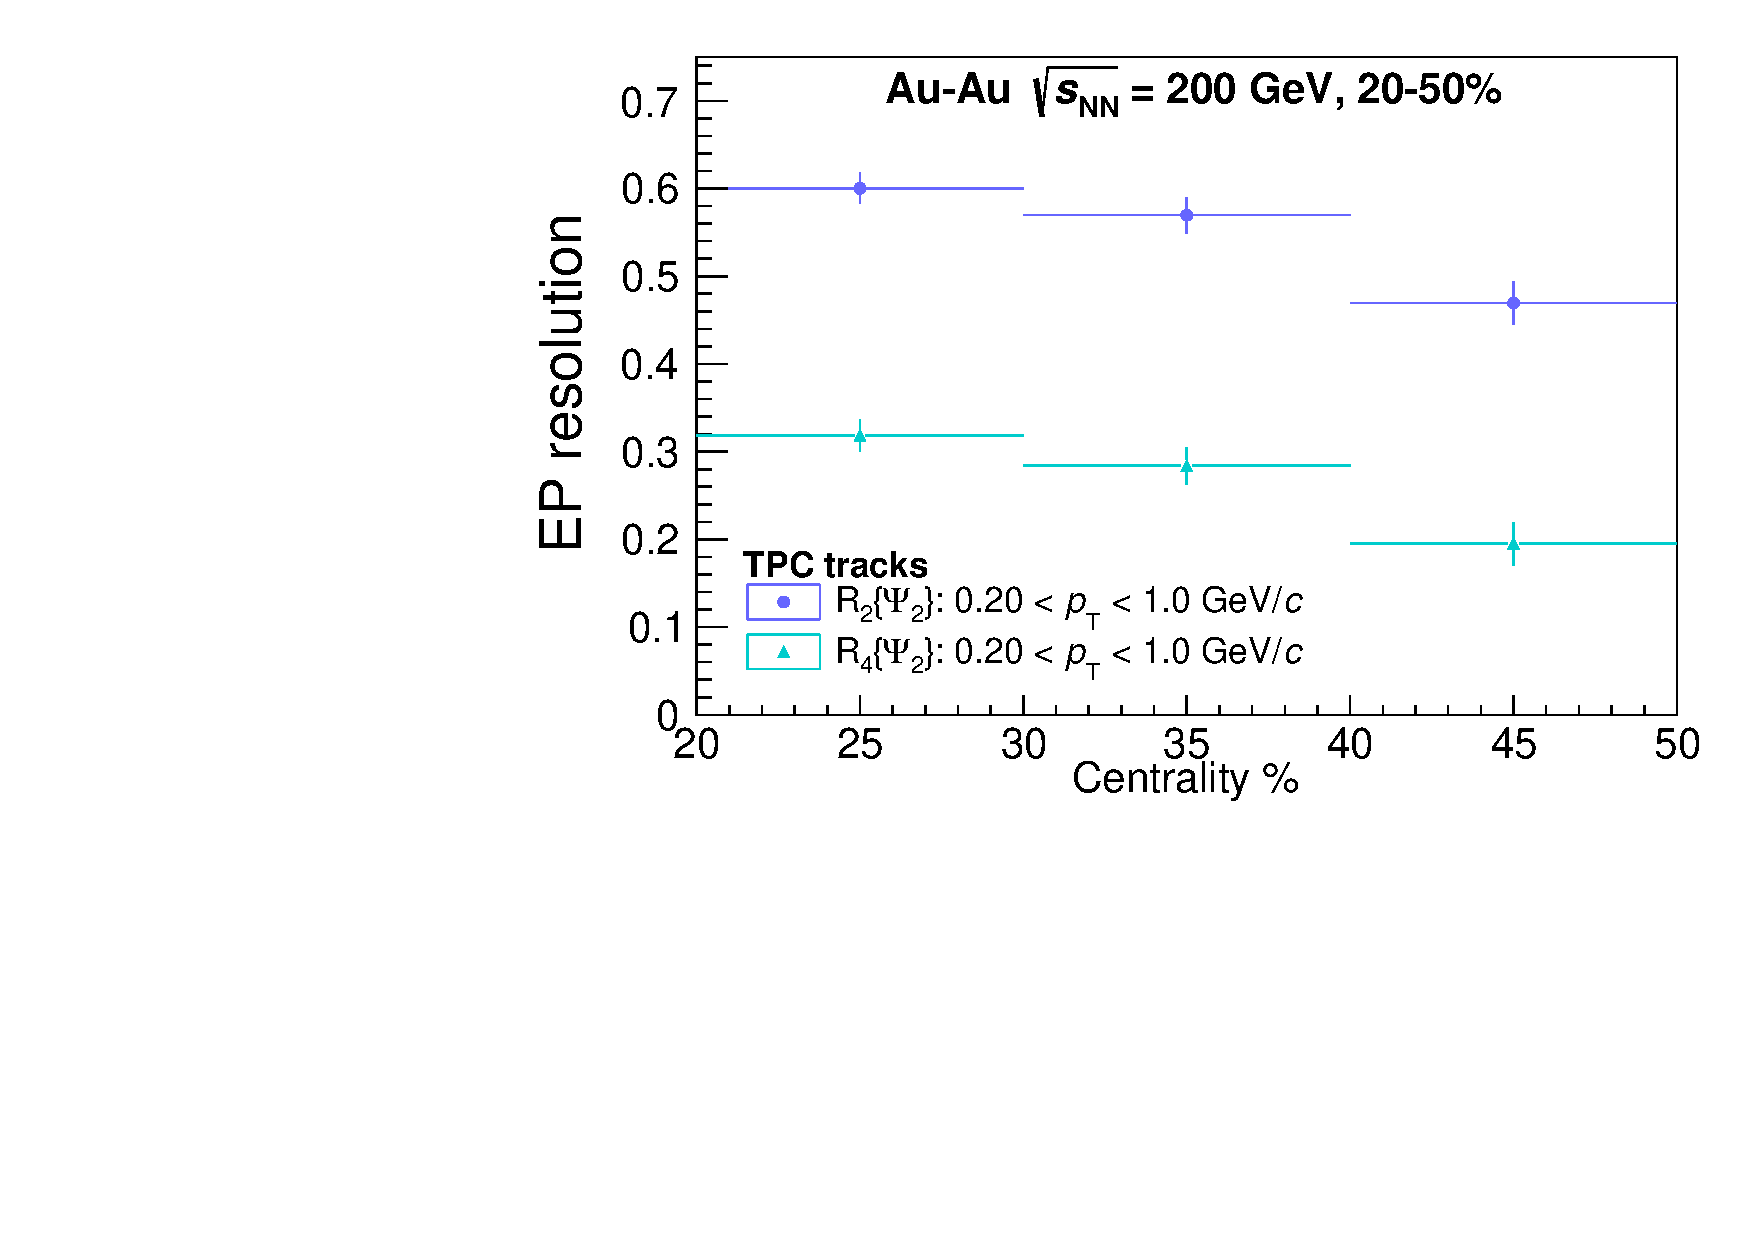
\includegraphics[width=12cm]{figures/R2-4combined.pdf}
		\caption[Event-plane resolution as a function of centrality]{Event-plane resolution: Second-order (fourth-order) harmonic relative to the event plane, $R_{2}(\Psi_{2})$ ($R_{4}(\Psi_{2})$), respectively.  The approach follows the Modified Reaction Plane (MRP) method \cite{Agakishiev:2014ada} utilizing the charged tracks of the TPC for event-plane reconstruction and resolution calculation for tracks with 0.2--1.0~\GeVc. Combined over 20--50\% centrality, $R_2 = 0.56$ and $R_4 = 0.28$. }  
		\label{fig:EPres}
	\end{center}
\end{figure}

Because the jets are sorted into the orientation bins with the reconstructed event plane, some in-plane jets are counted as mid- or out-of-plane and vice versa, which reduces any event-plane dependence of the signal.
%
This effect is not corrected for, since an unfolding of the orientation bins, or a Fourier decomposition of the signal, would require a precision the measurement does not have and would add further uncertainties.
%
Its size can instead be estimated with a simple model.
%
Suppose that path-length dependent jet quenching makes the associated yield per jet depend on the angle \(\Delta = \phi_\mathrm{jet} - \Psi_2\) between the jet and the \emph{true} symmetry plane as \(Y(\Delta) \propto 1 + 2 v_2^\mathrm{quench}\cos(2\Delta)\).
%
The coefficient $v_2^\mathrm{quench}$ is then the relative amplitude of this variation, in analogy with the flow coefficients of Sec.~\ref{sec:flowIntro}: for $v_2^\mathrm{quench} > 0$, in-plane jets, which traverse less medium, have larger associated yields than out-of-plane jets.
%
Measured relative to the reconstructed event plane, the variation is smeared, and its amplitude is reduced to $R_2 v_2^\mathrm{quench}$ (App.~\ref{sec:EP_Recon}).
%
Averaging $Y$ over the orientation bins of Eq.~\ref{Eq:EPbins} then gives, to first order in $v_2^\mathrm{quench}$, $Y_\mathrm{out}/Y_\mathrm{in} \approx 1 - (6\sqrt{3}/\pi) R_2 v_2^\mathrm{quench}$ and $Y_\mathrm{mid}/Y_\mathrm{in} \approx 1 - (3\sqrt{3}/\pi) R_2 v_2^\mathrm{quench}$.
%
The size of $v_2^\mathrm{quench}$ for the associated yields has not been measured.
%
As an illustration, $v_2^\mathrm{quench} = 0.1$ is taken, the upper end of the azimuthal anisotropy of the jet yields themselves measured at the LHC, between a few percent and about 0.1~\cite{ALICE:2015efi,ATLAS:2021ktw}, which arises from the same path-length dependence; whether the associated yields vary as strongly is not known.
%
With this value, the out-of-plane to in-plane (mid-plane to in-plane) yield ratio would be 0.67 (0.83) with a perfect event plane, but only 0.81 (0.91) with $R_2 = 0.56$, i.e.\ only about half of a real deviation from unity would remain visible.
%
The finite resolution therefore pulls any event-plane dependence of the yields toward unity, which must be kept in mind when interpreting the yield ratios in Sec.~\ref{sect:YieldRatio}.


\subsection{Jet reconstruction and selection} \label{sec:JetRecoAuAu}
Full jets are reconstructed by measuring charged tracks in the TPC and collecting neutral-particle information from the BEMC.  The anti-\kt algorithm 
%\cite{Cacciari:2008gp} implemented through the FastJet package \cite{Cacciari:2011ma} 
clusters these particles into jets by reconstructing the jet momenta as the quadratic sum of their constituent momenta using a boost-invariant $\it{p}^{2}_{\rm T}$ recombination scheme (Sec.~\ref{sec:jetAlgo}).  This scheme weights the directions of the constituents by $p^{2}_{\rm T}$ when they are combined, so that the jet axis follows the hardest constituents and is less sensitive to soft particles from the underlying event and from the recoil of the medium.  Tracks used for reconstructing jets are assumed to be pions while the towers to have arisen from massless particles. All jets measured in this work are clustered with resolution parameter of $R=0.4$. The area of jets, $A_{\rm jet}$, is found with FastJet using active ghost particles \cite{Cacciari:2008gn}.  Partially reconstructed jets at the edge of the acceptance are rejected by applying a fiducial cut, $|\eta_{\rm jet}| < 1.0 - R$, to assure all jets fall within the acceptance of the detectors. 

%This procedure uses the FastJet package \cite{Cacciari:2011ma}, where the anti-\kt \cite{Cacciari:2008gp} recombination algorithm is used for reconstructing signal jets and the \kt sequential recombination algorithm is used for estimating the underlying event background ($\rho$).  The momenta of the jet is calculated as the quadratic sum of their constituent momenta using a boost-invariant $\it{p}^{2}_{\rm T}$ recombination scheme.  Tracks used for reconstructing jets are assumed to be pions while the towers to have arisen from massless particles.  A jet can further be described by its resolution parameter $R$, which refers to its radial extension in azimuth and pseudorapidity.  The exact meaning of R is algorithm specific, but in this paper, it will typically refer to roughly circular clusters of radius R about the jet axis determined by $\Delta R = \sqrt{\dphi^2 + \deta^2}$ where \dphi (\deta) is the relative azimuthal angle (relative pseudorapidity).  The area of jets, $A^{jet}$, is found within the FastJet package utilizing active ghost particles \cite{Cacciari:2008gn}.  The location of a jet is described by the `jet axis', which refers to the azimuthal and pseudorapidity coordinates of the centroid of the jet.  Partially reconstructed jets at the edge of the acceptance are rejected by a fiducial cut, $|\eta_{jet}| < 1.0 - R$, to assure jets fall within the acceptance of the detectors.

Jets produced in heavy-ion collisions sit on top of a large amount of underlying event.  The jet signal can be found beneath tens to hundreds of particles resulting from various other processes. To reduce the influence of these background particles, this analysis requires tracks (towers) with $\ensuremath{p_{\rm T}}\xspace (\Et) >$ 2.0 \GeVc for jet reconstruction.  At RHIC energies this selection reduces the median background transverse-momentum density per unit $A_{\rm jet}$, $\langle \rho \rangle$, down to $\approx 0.6$~\GeVc.  This high-constituent selection, referred to as a ``hard-core'' jet selection, reduces fluctuations, fake jets, and background jet particles~\cite{PhysRevLett.119.062301}.  To further reduce contributions from the background and to match the trigger condition, the jets are required to contain a constituent tower that fired the HT trigger ($ E_{\rm T, tower}> 5.4$~GeV). Jets containing a track with $\ensuremath{p_{\rm T}}\xspace > 30$~\GeVc are rejected, as such tracks are likely to be mis-reconstructed. The remaining jets are studied in classes of jets with \pttrigrange{15}{20} and \pttrigrange{20}{40}.
%
The numbers of trigger jets in the two classes are shown in Fig.~\ref{fig:NTrig} for each orientation relative to the event plane.
%
There are about 31\,000 trigger jets with \pttrigrange{15}{20} in 20--50\% central collisions, and more jets are found in-plane than out-of-plane.
%
This ordering is expected both from the path-length dependence of jet quenching and from the larger in-plane background, which adds more momentum to in-plane jets and moves more of them above the selection threshold; the latter effect is addressed by the jet-energy-shift correction (Sec.~\ref{sect:SysUnc}).

\begin{figure}[!htbp]
	\centering
	\begin{tabularx}{\textwidth}{XX}
		\includegraphics[width=\linewidth]{JHC/NTrig_J15-20_C20-50_Zcut24.pdf} &
		\includegraphics[width=\linewidth]{JHC/NTrig_J20-40_C20-50_Zcut24.pdf} \\
	\end{tabularx}
	\caption[Number of trigger jets for each orientation relative to the event plane]{Number of trigger jets as a function of the reconstructed \Pt{jet} for \pttrigrange{15}{20} (left) and \pttrigrange{20}{40} (right) full jets in 20--50\% central \AuAu collisions, for in-plane (blue), mid-plane (magenta) and out-of-plane (red) jets and all orientations combined (black).}
	\label{fig:NTrig}
\end{figure}

No event-by-event subtraction of the underlying event, $\rho A_{\rm jet}$, is applied to the jet momenta: with 2~\GeVc constituents, too few background \kt jets are found in an event to estimate $\rho$ reliably, and the remaining background contribution is small.
%
The residual background and its dependence on the jet orientation relative to the event plane are instead accounted for by the jet-energy-shift correction described in Sec.~\ref{sect:SysUnc}.
%
The hard-core and trigger-tower requirements select jets that fragmented hard and lost little energy, which favors jets produced close to the surface of the medium and heading outward.
%
This \emph{surface bias} of the trigger jet increases, on average, the path length of the recoiling away-side jet through the medium.

\subsection{Jet-hadron correlation} \label{sect:Correlations}
The measurement of the correlation function (distribution of charged hadrons relative to reconstructed jets) described in Eq.~\ref{Eq:JHCorrIntro} requires several corrections.  The correlation function is measured in pseudorapidity (\deta) and azimuth (\dphi) as: 

\begin{equation}
	\frac{1}{N_{\rm trig}} \frac{d^2N_{\rm assoc,jet}}{d\dphi d\deta} = \frac{1}{N_{\rm trig}} \frac{1}{\epsilon(\Pt{assoc}, \eta_{\rm assoc})} \frac{1}{a(\Pt{assoc}, \text{\dphi}, \text{\deta})}\left(\frac{d^2 N^{\rm meas}_{\rm assoc,jet}}{d\dphi d\deta} - \frac{d^2 N^{\rm bkgd}_{\rm assoc,jet}}{d\dphi d\deta}\right) .
	\label{Eqtn:CorrFunction}
\end{equation}

\begin{sidewaysfigure}
	\centering
	\begin{tabularx}{\textwidth}{XXX@{\hskip 0.5cm}XXX}
		%\hline
		\includegraphics[width=\linewidth]{JHC/J15-20_C20-50_raw2D_sig_in_Ass1.0-1.5_Zcut24.pdf} & \includegraphics[width=\linewidth]{JHC/J15-20_C20-50_raw2D_mix_in_Ass1.0-1.5_Zcut24.pdf} & \includegraphics[width=\linewidth]{JHC/J15-20_C20-50_raw2D_ratio_in_Ass1.0-1.5_Zcut24.pdf} &
		\includegraphics[width=\linewidth]{JHC/J15-20_C20-50_raw2D_sig_in_Ass1.5-2.0_Zcut24.pdf} & \includegraphics[width=\linewidth]{JHC/J15-20_C20-50_raw2D_mix_in_Ass1.5-2.0_Zcut24.pdf} & \includegraphics[width=\linewidth]{JHC/J15-20_C20-50_raw2D_ratio_in_Ass1.5-2.0_Zcut24.pdf} \\
		\multicolumn{3}{c}{(a)}&\multicolumn{3}{c}{(b)}\\
		\multicolumn{6}{c}{}\\
		%\hline
		\includegraphics[width=\linewidth]{JHC/J15-20_C20-50_raw2D_sig_in_Ass2.0-3.0_Zcut24.pdf} & \includegraphics[width=\linewidth]{JHC/J15-20_C20-50_raw2D_mix_in_Ass2.0-3.0_Zcut24.pdf} & \includegraphics[width=\linewidth]{JHC/J15-20_C20-50_raw2D_ratio_in_Ass2.0-3.0_Zcut24.pdf} &
		\includegraphics[width=\linewidth]{JHC/J15-20_C20-50_raw2D_sig_in_Ass3.0-4.0_Zcut24.pdf} & \includegraphics[width=\linewidth]{JHC/J15-20_C20-50_raw2D_mix_in_Ass3.0-4.0_Zcut24.pdf} & \includegraphics[width=\linewidth]{JHC/J15-20_C20-50_raw2D_ratio_in_Ass3.0-4.0_Zcut24.pdf} \\
		\multicolumn{3}{c}{(c)}&\multicolumn{3}{c}{(d)}\\
		\multicolumn{6}{c}{}\\
		%\hline
		\includegraphics[width=\linewidth]{JHC/J15-20_C20-50_raw2D_sig_in_Ass4.0-6.0_Zcut24.pdf} & \includegraphics[width=\linewidth]{JHC/J15-20_C20-50_raw2D_mix_in_Ass4.0-6.0_Zcut24.pdf} & \includegraphics[width=\linewidth]{JHC/J15-20_C20-50_raw2D_ratio_in_Ass4.0-6.0_Zcut24.pdf} &
		\includegraphics[width=\linewidth]{JHC/J15-20_C20-50_raw2D_sig_in_Ass6.0-10.0_Zcut24.pdf} & \includegraphics[width=\linewidth]{JHC/J15-20_C20-50_raw2D_mix_in_Ass6.0-10.0_Zcut24.pdf} & \includegraphics[width=\linewidth]{JHC/J15-20_C20-50_raw2D_ratio_in_Ass6.0-10.0_Zcut24.pdf}\\
		\multicolumn{3}{c}{(e)}&\multicolumn{3}{c}{(f)}\\
		%\hline
	\end{tabularx}
%		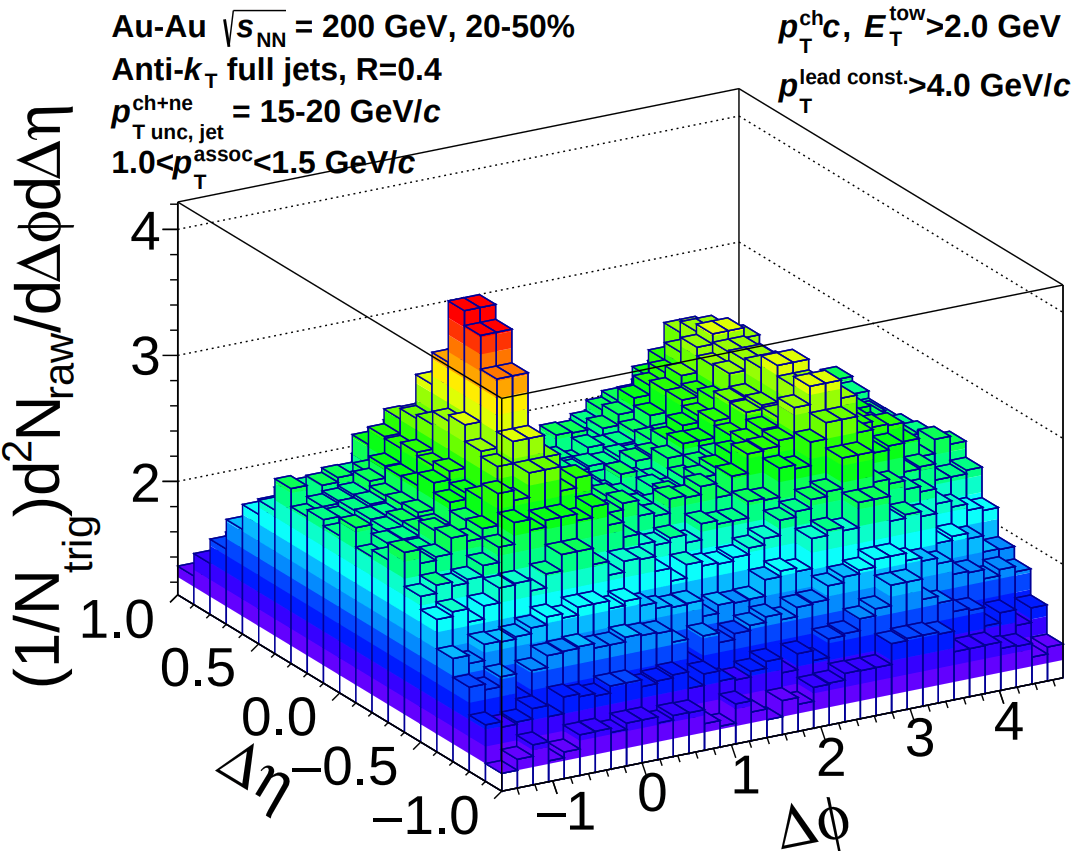
\includegraphics[width=0.49\linewidth]{figures/jhcorr_jpt1520}
%	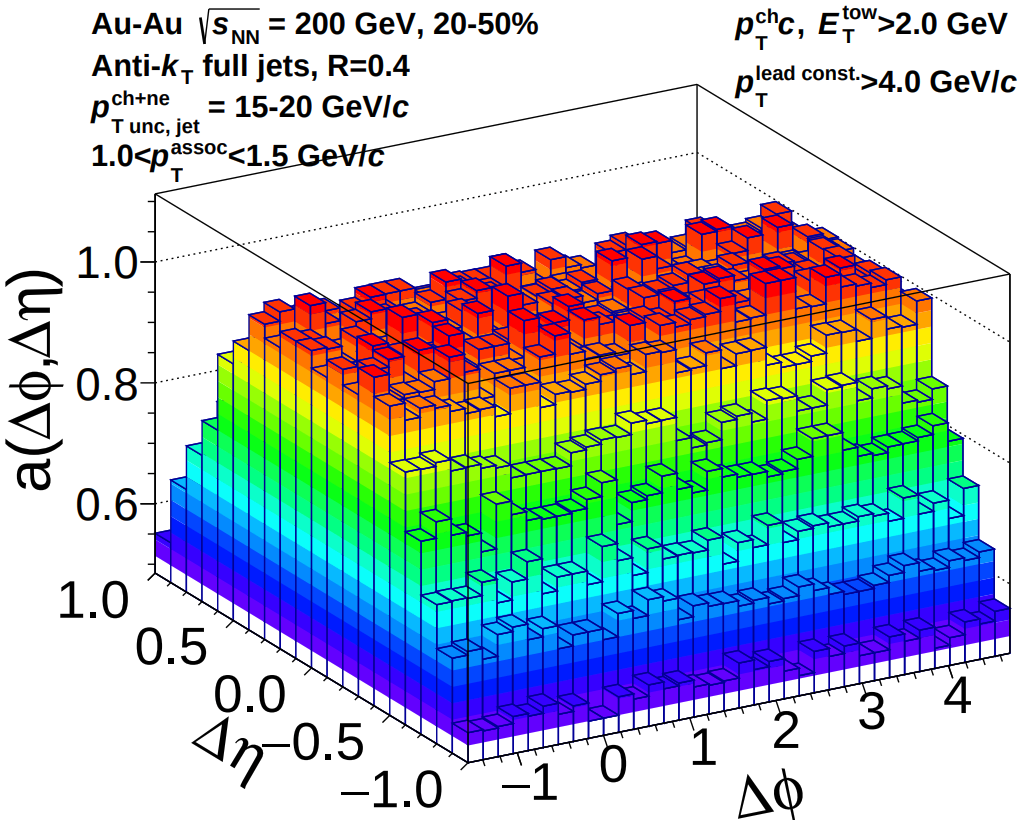
\includegraphics[width=0.49\linewidth]{figures/ajhcorr_jpt1520}
	\caption[Raw, mixed-event and acceptance-corrected jet-hadron correlations for 15--20~GeV/\(c\) jets]{Two-dimensional jet-hadron correlations in \dphi and \deta for in-plane \pttrigrange{15}{20} jets in 20--50\% central \AuAu collisions, for the associated-hadron momenta (a) \ptassocrange{1.0}{1.5}, (b) \ptassocrange{1.5}{2.0}, (c) \ptassocrange{2.0}{3.0}, (d) \ptassocrange{3.0}{4.0}, (e) \ptassocrange{4.0}{6.0} and (f) \ptassocrange{6.0}{10.0}. Each group shows, from left to right, the raw same-event distribution per trigger jet, the normalized mixed-event pair acceptance $a(\dphi, \deta)$, whose trapezoidal shape in \(\Delta\eta = \eta_\mathrm{jet} - \eta_\mathrm{assoc}\) follows from \(|\eta_\mathrm{assoc}| < 1.0 \) and \(|\eta_\mathrm{jet}| < 0.6 \), and the acceptance-corrected correlation function, which still contains the combinatorial background.}
	\label{fig:jhcorrjpt1520}
\end{sidewaysfigure}

%\noindent where and acceptance, $a(\dphi, \deta)$ is the acceptance correction for track pairs, $N_{meas}$ is the measured number of associated particles, and $N_{bkgd}$ is the number of associated particles from the background.  The single-track reconstruction efficiency and acceptance only account for the reconstruction of associated particles.
%\begin{equation}
%   C(\dphi, \deta)= \frac{  \frac{d^2 N^{same}_{pair}}{d\dphi 
		%   d \deta}} {  \frac{d^2 N^{mixed}_{pair}}{d \dphi d \deta}}
%   \label{Eqn:correlationfnc}
%\end{equation}

%and express our associated per trigger yield by:

%\begin{equation}
%  \frac{d^2 N}{d\dphi d\deta}(\dphi,\deta,\Delta\Psi_{RP,2}) = \frac{1}{N_{trig}} %\frac{dN_{assoc}}{d\dphi d\deta}
%  \label{Eqn:correlationfncPerTrig}
%\end{equation}

Here, $N_{\rm assoc, jet}$ gives the number of pairs of trigger jets and the associated hadrons, $N^{\rm meas}_{\rm assoc,jet}$ and $N^{\rm bkgd}_{\rm assoc,jet}$ are the number of pairs measured and the pair characterized as background respectively. The single-track reconstruction efficiency is $\epsilon(\Pt{assoc}, \eta_{\rm assoc})$\footnote{Acceptance effects such as gaps between sector boundaries are included in this correction; however, $\epsilon(\Pt{assoc}, \eta_{\rm assoc})$ is referred to as an efficiency correction in order to distinguish it from $a(\Pt{assoc}, \text{\dphi}, \text{\deta})$.}.  The pair acceptance, $a(\Pt{assoc}, \text{\dphi}, \text{\deta})$, is calculated from the raw pairs measured between a trigger jet and the charged hadrons from mixed events.  %The background correction $N_{\rm bkgd}$ is described in Sec.~\ref{sect:CorrBkgd}.

The correlations are determined in bins of centrality, reconstructed trigger-jet transverse momentum (\Pt{jet}), associated-hadron transverse momentum (\Pt{assoc}), and bins of the trigger jet relative to the event plane (in, mid, out, all combined angles) defined in Eq.~\ref{Eq:EPbins}.  Fig.~\ref{fig:jhcorrjpt1520} shows, for in-plane \pttrigrange{15}{20} jets, how the raw same-event distributions are turned into acceptance-corrected correlation functions by the mixed-event correction described below.  The corrected correlation functions contain a large combinatorial background ($N^{\rm bkgd}_{\rm assoc,jet}$), which must be subtracted.  This subtraction procedure is described in Sec.~\ref{sect:CorrBkgd}.

%The acceptance correction is applied in \dphi and \deta before further analysis and background subtraction.  Figure shows an example of the raw correlations from same events pairs before applying a mixed event correction for the efficiency and acceptance of the BEMC.  A plateau structure can be seen due to the finite acceptance of track pairs.


%=============================================================
%=============================================================
\subsubsection{Pair-acceptance correction from mixed events}
\label{sect:MixedEvents}
% Mixed events should not contain physics correlations, but information of the acceptance and efficiency of single event pairs.

The pair-acceptance correction, $1 / a(\Pt{assoc}, \text{\dphi}, \text{\deta})$, accounts for the detector and tracking inefficiencies, and is found by correlating jets from HT-triggered events with associated hadrons from MB events of the same event class. %(centrality, primary vertex position in the z-direction).  
%
In addition to providing the acceptance correction, the mixed-event procedure will also help remove the trivial correlation due to an $\eta$ dependence in the single-particle track distributions~\cite{PhysRevC.101.064901}.  
%
Taking the ratio of the same-event pairs to the mixed-event pairs removes the detector effects of acceptance and efficiency.  
%
The pair acceptance will serve as the dominant effect, given that there is little $\eta$ dependence in both the tracks and jets across the acceptance range of this analysis.
%
Since the trigger jets are restricted to $|\eta_\mathrm{jet}| < 0.6$ and the associated hadrons to $|\eta_\mathrm{assoc}| < 1.0$, the number of possible pairs is constant for $|\deta| < 0.4$ and falls linearly to zero at $|\deta| = 1.6$, which gives the pair acceptance its trapezoidal shape in \deta, illustrated with a toy model in Fig.~\ref{fig:ToyMixedEvent} and visible in the measured mixed-event distributions of Fig.~\ref{fig:jhcorrjpt1520}.
%
Because the trigger jet and the associated hadrons of a mixed pair come from different events, they are correlated only through this acceptance.

\begin{figure}[!htbp]
	\centering
	\includegraphics[width=0.6\linewidth]{JHC/ToyMixedEventModel-eps-converted-to.pdf}
	\caption[Toy model of the pair acceptance in \(\Delta\eta\)]{Toy model of the pair acceptance in $\deta = \eta_\mathrm{jet} - \eta_\mathrm{hadron}$ for uncorrelated trigger jets and hadrons, each uniformly distributed in pseudorapidity (here $|\eta_\mathrm{jet}| < 0.5$ and $|\eta_\mathrm{hadron}| < 0.9$). The number of pairs is constant where the smaller acceptance is fully contained in the larger one and falls linearly to zero at the largest possible separation. The analysis uses the plateau region $|\deta| < 0.4$ to normalize the measured mixed-event distributions.}
	\label{fig:ToyMixedEvent}
\end{figure}


%To increase the sampling size of mixed events used for the acceptance correction, both MB30 and MB5 triggered events are used for event mixing.  After re-weighting the reference multiplicity distributions to correct for the VPD trigger inefficiency, MB5 events are added with an additional weight factor such that they are normalized to MB30 events in a 2-dimensional fashion to account for VPD resolution differences across centrality and the online VPD vertex cut which had a negative $v_z$ offset.  Additional details can be found in Ref.~\cite{PhysRevC.99.034908}.  

The event mixing follows Ref.~\cite{PhysRevC.96.024905}. The MB events are kept in pools binned in 10\% centrality and 4-cm $v_z$ intervals, each holding up to 25\,000 tracks; each trigger jet is correlated with the tracks of all events in the pool of its event class, and the mixed-event pairs are weighted by the inverse of the number of mixed events. The acceptance is constructed separately for the 20--30\%, 30--40\%, and 40--50\% centrality classes and then combined.  High-momentum tracks are nearly straight, so the detector acceptance does not change significantly at high-\Pt{assoc}, and thus all associated momentum bins greater than 2.0 \GeVc are combined to increase statistics.  There is no difference in efficiency and acceptance within uncertainties for different orientations of the jet relative to the event plane, and therefore the same correction $a(\Pt{assoc}, \text{\dphi}, \text{\deta})$ is applied for all angles relative to the event plane.  The acceptance $a(\Pt{assoc}, \text{\dphi}, \text{\deta})$ is normalized to 1 at its maximum, determined using the region of approximately constant acceptance ($|\deta| <$ 0.4).  For each \Pt{assoc} bin, the projection of the flat plateau region (integrated over the region $|\deta| <$ 0.4) was fit with a constant over the whole \dphi range.

\subsubsection{Uncertainties of the pair-acceptance correction}
\label{sect:MixedEventsUnc}
Three uncertainties are associated with the pair-acceptance correction: the normalization of the mixed events, and the shape of the correction in \dphi and in \deta that results from its dependence on the vertex position.
%
The uncertainties of the fits of the plateau were used for the systematic uncertainty on the mixed-event normalization, which is added in quadrature and reported as the scale uncertainty.  This systematic uncertainty is under 1\% (1.25\%) in all \Pt{assoc} bins used for the reported results of jets with  \pttrigrange{15}{20} and  \pttrigrange{20}{40}.

A shape uncertainty in \dphi due to the \zvtx binning, similar to that in \deta, could lead to an additional shape uncertainty in the correlation functions.  To test for this, the ratio of the 1D \dphi projection with the nominal \zvtx binning and the binning described above was calculated for each \Pt{jet}, \Pt{assoc}, and centrality bin.  The variations about 1.0 are smaller than the statistical errors associated with the points.  This uncertainty was therefore considered negligible.

There is an additional shape uncertainty associated with the application of the acceptance correction due to slight changes in the correlation function at large \deta in the acceptance with $v_z$ position.  The background level is determined from the level of the correlation function at large \deta, leading to a scale uncertainty in the background subtraction dependent on \Pt{assoc}.  This uncertainty is from the differences between the nominal (z-integrated) and the z-vertex method (z-binned) for correcting the mixed events on the level of the background in the $0.6 < \deta < 1.2$ range, and signal plus background, in the $|\deta| < 0.6$ range.  The large \deta region is used to determine the background so any uncertainties in the level of the correlation function in this region lead to an uncertainty in the level of the background in the signal region.  This is expressed as an additional scale band on the final results.

In the nominal (z-integrated) method the same- and mixed-event distributions are summed over all $v_z$ bins before the division, because dividing the sample into 4-cm $v_z$ bins, as would be ideal given the $v_z$ dependence of the acceptance, enlarges the statistical fluctuations of the mixed-event normalization in each bin.
%
In the z-binned method the acceptance correction is instead applied separately in each bin $i$,
%
\begin{equation}
	\frac{1}{N_{\rm trig}} \frac{d^2N_{\rm assoc,jet}}{d\dphi d\deta} = \frac{1}{N_{\rm trig}} \sum_i \frac{1}{\epsilon\, a_i(\dphi, \deta)} \frac{d^2 N_i}{d\dphi d\deta},
	\label{Eqtn:CorrFunctionZbinned}
\end{equation}
%
where $N_i$ and $a_i$ are the same-event pairs and the pair acceptance in $v_z$ bin $i$.
%
For each method, the ratio of the integrals of the correlation function $Y$ over the signal+background ($|\deta| < 0.6$) and background-dominated ($0.6 < |\deta| < 1.2$) regions is computed, and their ratio defines the scale factor
%
\begin{equation}
	\alpha = \frac{\int_\mathrm{sig} Y_\mathrm{nom}\, d\deta \Big/ \int_\mathrm{bkgd} Y_\mathrm{nom}\, d\deta}{\int_\mathrm{sig} Y_{z\mathrm{vtx}}\, d\deta \Big/ \int_\mathrm{bkgd} Y_{z\mathrm{vtx}}\, d\deta}
	\label{Eqtn:alpha}
\end{equation}
%
for each \Pt{assoc} bin.
%
The scale band is obtained by multiplying the correlation function by $\alpha$ and by $2 - \alpha$.
%
This uncertainty is determined by varying the binning of the mixed events in $v_z$ and is correlated for different angles relative to the event plane and for different bins in \Pt{assoc}.  For $\Pt{assoc} >$ 3~\GeVc, this uncertainty is negligible because the background is small.

\subsection{Flow modulation of combinatorial background} \label{sect:CorrBkgd}
The combinatorial background ($N^{\rm bkgd}_{\rm assoc,jet}$) from Eq.~\ref{Eqtn:CorrFunction} can be parametrized for trigger jets restricted to the orientation $\mathfrak{R} = {\text{in/mid/out-of-plane}}$ relative to the event plane as~\cite{Bielcikova:2003ku,Sharma:2015qra}:

\begin{equation}
	\left(\frac{1}{\pi}\frac{dN^{\rm bkgd}_{\rm assoc,jet}}{d\dphi}\right)_\mathfrak{R} = B^\mathfrak{R}\left( 1 + \sum_{n=2}^{\infty} 2 v_{n,\mathrm{assoc}} v^\mathfrak{R}_{n, \mathrm{jet}} \cos(n\dphi)\right)
	\label{Eqtn:JBBBCorrelations},
\end{equation}

\noindent where $v_{n,\mathrm{assoc}}$ and $v^\mathfrak{R}_{n, \mathrm{jet}}$ are the Fourier coefficients of the azimuthal angle distribution (flow coefficients) of background associated particles and trigger jets restricted to the orientation $\mathfrak{R}$ respectively. The factor $B^\mathfrak{R}$ gives the background level amplitude for orientation $\mathfrak{R}$. The trigger jets being restricted to orientation $\mathfrak{R}$ modifies their nominal flow coefficients $v_{n, \mathrm{jet}}$'s into the $v^\mathfrak{R}_{n, \mathrm{jet}}$ from Eq.~\ref{Eqtn:JBBBCorrelations} which are related to each other as ~\cite{Bielcikova:2003ku}:

\begin{equation}
	v^{\mathfrak{R}}_{n, \mathrm{jet}} = 
	\begin{cases}
		\frac{v_{n, \mathrm{jet}}}{\beta^\mathfrak{R}}+ \cos(n\phi_{s}^\mathfrak{R}) \frac{\sin(nc)}{nc}\frac{R_{n}}{\beta^\mathfrak{R}} + &\\
		\frac{1}{\beta^\mathfrak{R}}\sum_{k=2,4,6,..} (v_{(k+n), \mathrm{jet}}+v_{|k-n|, \mathrm{jet}})
		\cos(k\phi_{s}^\mathfrak{R}) \frac{\sin(kc)}{kc}R_{k} & \text{if $n$ is even,}\\
		v_{n, \mathrm{jet}} & \text{if $n$ is odd.}
	\end{cases},
	\label{Eq:vRn}
\end{equation}
where, $\beta^\mathfrak{R}$ is the $\mathfrak{R}$ dependence of $B^\mathfrak{R}$ given by,
\begin{equation}
	B^\mathfrak{R} \propto \beta^\mathfrak{R} = 1 + \sum_{k=2,4,6,..} 2v_{k, \mathrm{jet}} \cos(k\phi_{s}^\mathfrak{R}) \frac{\sin(kc)}{kc}R_{k}.
	\label{Eq:betaR}
\end{equation}
Here $\phi_S^\mathfrak{R}$ and $c$ are the center and half-width of the $|\Psi_{2,EP}-\phi_{\mathrm {jet}}|$ range for jets restricted to orientation $\mathfrak{R}$. The \(R_n\) and \(R_k\) are the event-plane resolutions of Fig.~\ref{fig:EPres}; through them, the background parametrization accounts for the smearing of the jet orientations by the finite resolution, so that the background subtraction is corrected for it (Sec.~\ref{sec:EPReco}). Odd $v_{n, \mathrm{jet}}$'s mainly arise from initial state fluctuations and are therefore uncorrelated with the second-order event-plane and remain constant when the trigger jet is moved relative to the event plane, while even $v_{n, \mathrm{jet}}$'s will change~\cite{Aad:2014fla,Sharma:2015qra}. The $\mathfrak{R}$ dependent background shape is dependent upon the event-plane resolutions ($R_{n}$), which are fixed at the measured values (Sec.~\ref{sect:Method}). Further details of the derivations can be found in Refs.~\cite{Bielcikova:2003ku,Nattrass_2018,Nattrass_Reexam2018}. 

%The correlation function will contain contributions from all physical correlations in the event.  Quantum correlations between particles from the same source, known as Hanbury-Brown-Twiss (HBT) correlations, are suppressed by a difference between the momentum of the trigger and associated particles \cite{Lisa_2005}.  The \vneffnot of Eq.~\ref{Eqtn:JBBBCorrelations} may arise due to hydrodynamical flow or jet quenching.  When fixing a trigger (jet) relative to the event plane, the level of the background and effective $v_{n}^{t}$ are modified \cite{Bielcikova:2003ku}. for even $n$ $\tilde{v}^{R,t}_{n}$ can be reduced to:    

Collective particle flow plays a major role in understanding the underlying-event background.  This background consists of particles created from mechanisms unrelated to the hard process that led to a jet.  Some of the jet signal is correlated with the event plane due to the path-length dependence of partonic energy loss, while soft hadrons are predominantly correlated with the event plane due to hydrodynamical flow that also contribute to the bulk-particle production. 

\subsubsection{Reaction plane fit} \label{sect:RPF}
To remove the combinatorial background from the underlying event, the reaction plane fit (RPF) developed in Ref.~\cite{Sharma:2015qra} is applied in this work.
%
The measured jet-hadron correlation signal is decomposed into a \ns and an \as, with the former being narrow in \dphi and \deta and the latter narrow in \dphi, but broad in \deta.
%
The narrowness of the near-side implies the signal is negligible at large \deta, where the background dominates.
%
For the RPF, the `signal + background' region is defined as $|\deta| < 0.6$ and the background-dominated region, where the signal is assumed to be negligible, as $0.6 \leq |\deta| < 1.2$; the outermost \deta bins, up to $|\deta| = 1.6$, are not used because the small pair acceptance there makes the corrected correlation function fluctuate strongly.
%
The \dphi projection of the background-dominated region is fit with the parametrization of Eq.~\ref{Eqtn:JBBBCorrelations} over $|\dphi|<\pi/2$, where the away-side jet does not contribute, simultaneously for in-plane, mid-plane, and out-of-plane trigger jets.
%
The three orientations share the jet and associated-hadron flow coefficients, and their different background shapes (Eqs.~\ref{Eq:vRn} and~\ref{Eq:betaR}) constrain the fit much more strongly than a fit to a single orientation would.
%
The correlation function for all orientations combined is not included in the fit, as it would double count the same pairs.
%
The fitted background is then extrapolated over the full \dphi range and subtracted from the signal+background region.

RPF improves upon prior background subtraction techniques~\cite{PhysRevC.101.064901,Nattrass:2016cln} by avoiding problems due to contamination from jets on both the near- and away-side by using the \ns at large \deta and also using the dependence of the flow-modulated background on the angle of the trigger jet relative to the event plane to constrain the background shape and level. %The RPF method was used in a re-analysis of STAR data in Ref.\cite{} and further by the ALICE Collaboration in Ref., .  

The fits include the terms up to $n = 4$.
%
At high \Pt{assoc} the combinatorial background is small and few tracks are found at large \deta from the trigger jet, so the higher-order terms can no longer be constrained and the fit is restricted to $n = 3$; this is the case for $\Pt{assoc} > 4$~\GeVc with \pttrigrange{15}{20} jets and $\Pt{assoc} > 3$~\GeVc with \pttrigrange{20}{40} jets.
%
Therefore, the RPF fits consist of six parameters ($B$, $v_{2, \rm jet}$, $v_{2, \mathrm {assoc}}$, $(v_{3, \mathrm {jet}}\times v_{3, \mathrm {assoc}})$, $v_{4, \mathrm {jet}}$, and $v_{4, \rm assoc}$) for low \Pt{assoc}, and four ($B$, $v_{2, \rm jet}$, $v_{2, \mathrm {assoc}}$ and $(v_{3, \mathrm {jet}}\times v_{3, \mathrm {assoc}})$) for high \Pt{assoc}, from which the orientation-dependent $B^\mathfrak{R}$ and $v^\mathfrak{R}_{n, \mathrm{jet}}$ follow.
%
The fits, with their quality shown as (data $-$ fit)/fit, are shown for \pttrigrange{15}{20} jets in Fig.~\ref{fig:RPFfitJ1520}, and the extracted background level and $v_{2,\mathrm{assoc}}$ are shown in Fig.~\ref{fig:RPFpars}.
%
The background level falls by more than three orders of magnitude between the lowest and the highest \Pt{assoc} bin, and the extracted $v_{2,\mathrm{jet}}$ and $v_{2,\mathrm{assoc}}$ are consistent with earlier STAR measurements of the jet and charged-hadron $v_2$, despite the differences in method and event selection.

The uncertainty of the background is obtained from the covariance matrix $\sigma_{ij}$ of the fit parameters $p_i$: for any quantity $f$ derived from the fitted background, such as the background in a \dphi bin or its integral,
%
\begin{equation}
	\sigma_f^2 = \sum_{i=0}^{N} \sum_{j=0}^{N} \frac{\partial f}{\partial p_i} \frac{\partial f}{\partial p_j} \sigma_{ij}.
	\label{eqn:CovProp}
\end{equation}
%
Since the three orientations are fit simultaneously, this uncertainty is correlated point-to-point in \dphi and between orientations.

\begin{figure}
	\centering
	\begin{tabularx}{\textwidth}{XX}
		\includegraphics[width=\linewidth]{JHC/FitPars_Background_J15-20_C20-50_Zcut24.pdf}&
		\includegraphics[width=\linewidth]{JHC/FitPars_Background_J20-40_C20-50_Zcut24.pdf}\\
		\includegraphics[width=\linewidth]{JHC/FitPars_v2Assoc_J15-20_C20-50_Zcut24.pdf}&
		\includegraphics[width=\linewidth]{JHC/FitPars_v2Assoc_J20-40_C20-50_Zcut24.pdf}\\
%		\includegraphics[width=\linewidth]{JHC/FitPars_v2Jet_J15-20_C20-50_Zcut24.pdf}&
%	%	\includegraphics[width=\linewidth]{JHC/FitPars_v3sq_J15-20_C20-50_Zcut24.pdf}&
%		\includegraphics[width=\linewidth]{JHC/FitPars_v4Assoc_J15-20_C20-50_Zcut24.pdf}&
%		\includegraphics[width=\linewidth]{JHC/FitPars_v4Jet_J15-20_C20-50_Zcut24.pdf}&\\
%%
%		\includegraphics[width=\linewidth]{JHC/FitPars_v2Jet_J20-40_C20-50_Zcut24.pdf}&
%		\includegraphics[width=\linewidth]{JHC/FitPars_v3sq_J20-40_C20-50_Zcut24.pdf}&
%		\includegraphics[width=\linewidth]{JHC/FitPars_v4Assoc_J20-40_C20-50_Zcut24.pdf}&
%		\includegraphics[width=\linewidth]{JHC/FitPars_v4Jet_J20-40_C20-50_Zcut24.pdf}
	\end{tabularx}
	\caption[Parameters of the RPF fits as a function of \(p_\mathrm{T, assoc}\)]{Parameters of the RPF fits as a function of \Pt{assoc} for \pttrigrange{15}{20} (left) and \pttrigrange{20}{40} (right) full jets in 20--50\% central \AuAu collisions: the background level $B$ (top) and the second-order flow coefficient of the associated hadrons, $v_{2,\mathrm{assoc}}$ (bottom). The fits are performed over $|\dphi| < \pi/2$ in the background-dominated region $0.6 < |\deta| < 1.2$.}
	\label{fig:RPFpars}
\end{figure}

\begin{sidewaysfigure}
	\centering
		% OLD \includegraphics[width=16cm]{figures/plots/physics/PWfitBgExtract_A1.0-1.5_Trig15-20_C20-50_Zcut24.pdf}
	\begin{tabularx}{\textwidth}{XX}
		(a) & (b) \\
		\includegraphics[width=\linewidth]{JHC/JHCorrBGsub_A1.0-1.5_T15-20_C20-50.pdf} &
		\includegraphics[width=\linewidth]{JHC/JHCorrBGsub_A1.5-2.0_T15-20_C20-50.pdf} \\
		(c) & (d) \\
		\includegraphics[width=\linewidth]{JHC/JHCorrBGsub_A2.0-3.0_T15-20_C20-50.pdf} &
		\includegraphics[width=\linewidth]{JHC/JHCorrBGsub_A3.0-4.0_T15-20_C20-50.pdf} \\
		(e) & (f) \\
		\includegraphics[width=\linewidth]{JHC/JHCorrBGsub_A4.0-6.0_T15-20_C20-50.pdf} &
		\includegraphics[width=\linewidth]{JHC/JHCorrBGsub_A6.0-10.0_T15-20_C20-50.pdf} \\
	\end{tabularx}
		\caption[RPF background fits for 15--20~GeV/\(c\) jets]{RPF fits for \pttrigrange{15}{20} full jets in 20--50\% central \AuAu collisions, for (a) \ptassocrange{1.0}{1.5}, (b) \ptassocrange{1.5}{2.0}, (c) \ptassocrange{2.0}{3.0}, (d) \ptassocrange{3.0}{4.0}, (e) \ptassocrange{4.0}{6.0} and (f) \ptassocrange{6.0}{10.0}. Each panel shows, from left to right, in-plane, mid-plane and out-of-plane jets and all orientations combined. Upper panels: \dphi projections of the signal+background region ($|\deta| < 0.6$, green) and of the background-dominated region ($0.6 < |\deta| < 1.2$, black), with the RPF fit to the background-dominated region (blue band, fit uncertainty). Lower panels: quality of the fit to the background-dominated region, (data $-$ fit)/fit.}
		\label{fig:RPFfitJ1520}
\end{sidewaysfigure}

\begin{sidewaysfigure}
	\centering
%		\rotatebox{0}{\resizebox{\textwidth}{!}{
%				%         \includegraphics{figures/SampleCorrelation.pdf}
%				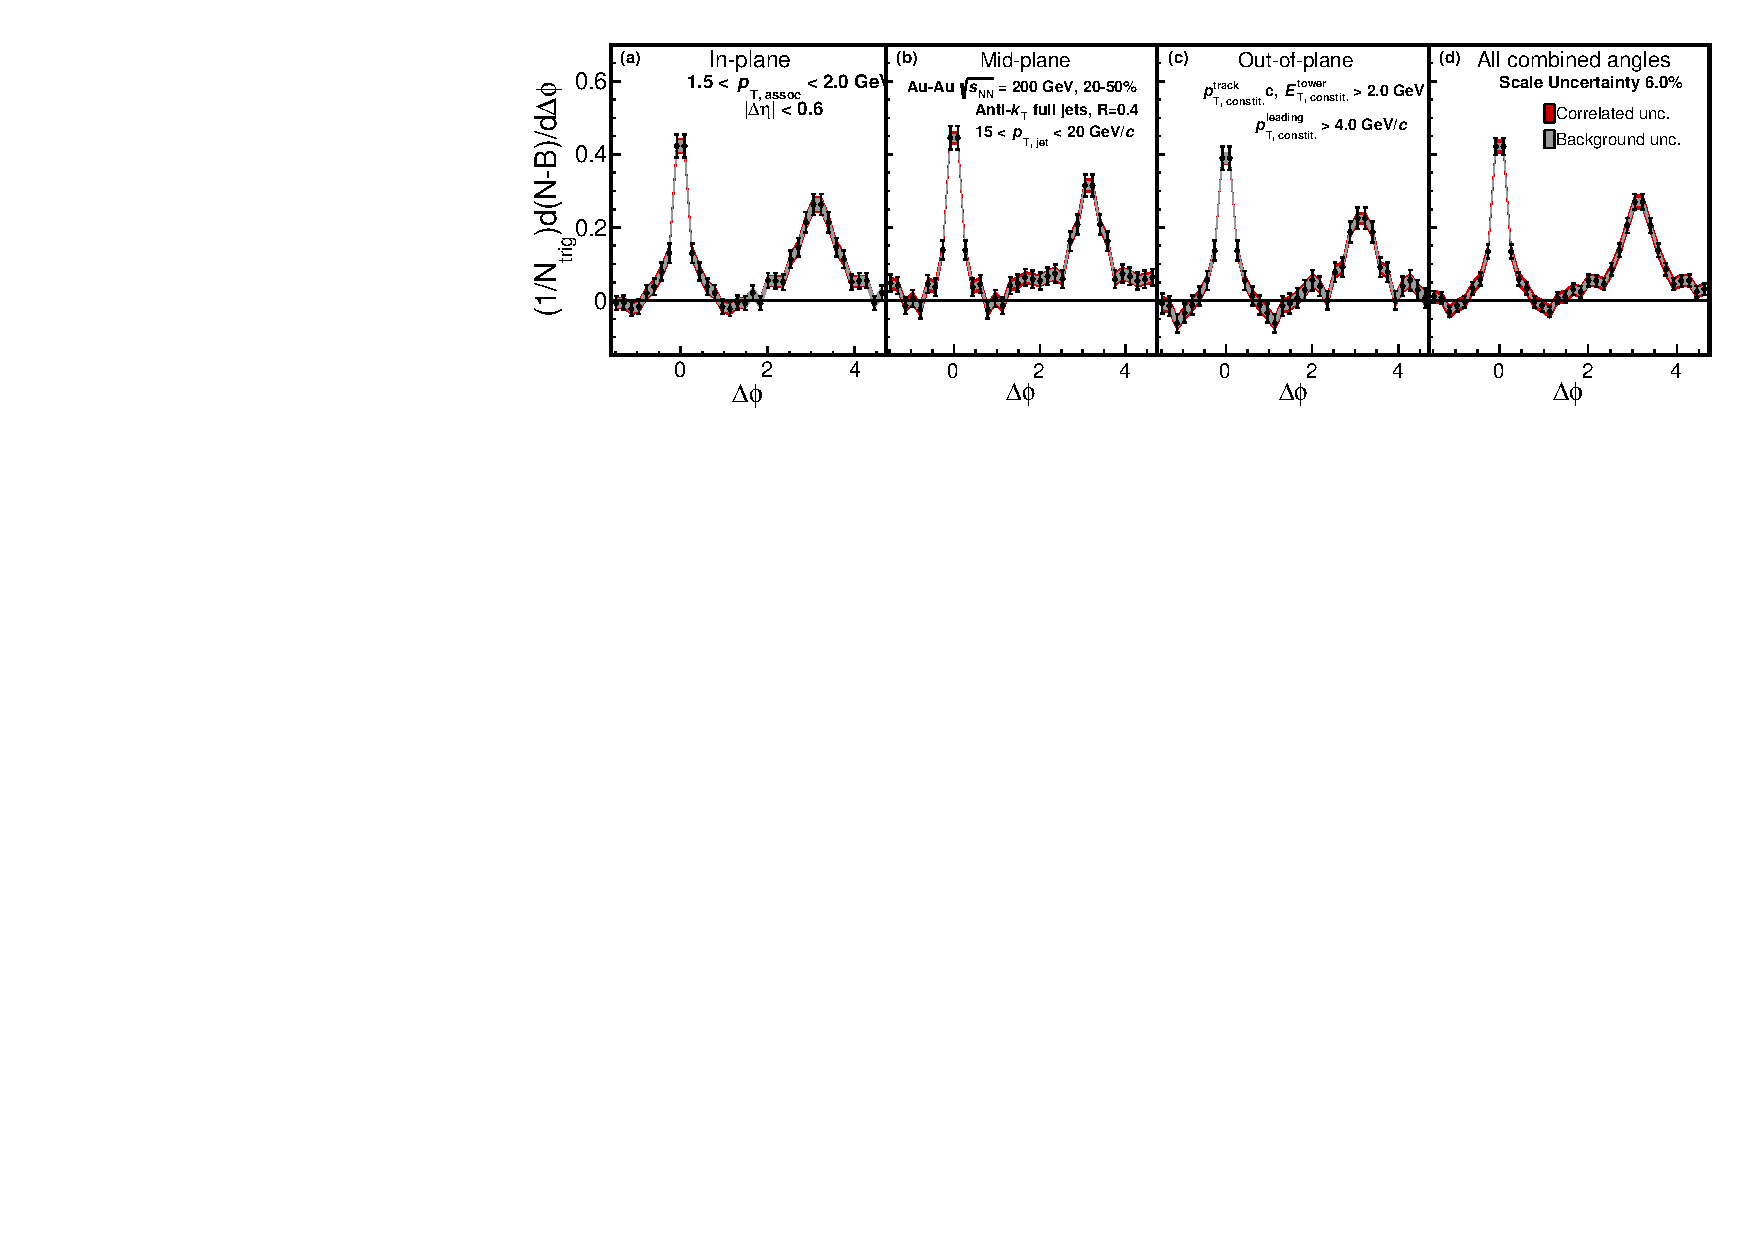
\includegraphics{figures/dPhiCorrelationsJ15-20_C20-50_1.5-2.0-paperplot.pdf}
%		}}
	\begin{tabularx}{\textwidth}{XX}
		(a) & (b) \\
	\includegraphics[width=\linewidth]{JHC/dPhiCorrelationsJ15-20_C20-50_1.0-1.5.pdf} &
	\includegraphics[width=\linewidth]{JHC/dPhiCorrelationsJ15-20_C20-50_1.5-2.0.pdf} \\
			(c) & (d) \\
	\includegraphics[width=\linewidth]{JHC/dPhiCorrelationsJ15-20_C20-50_2.0-3.0.pdf} &
	\includegraphics[width=\linewidth]{JHC/dPhiCorrelationsJ15-20_C20-50_3.0-4.0.pdf} \\
			(e) & (f) \\
	\includegraphics[width=\linewidth]{JHC/dPhiCorrelationsJ15-20_C20-50_4.0-6.0.pdf} &
	\includegraphics[width=\linewidth]{JHC/dPhiCorrelationsJ15-20_C20-50_6.0-10.0.pdf} \\
\end{tabularx}

		\caption[Background-subtracted jet-hadron correlations for 15--20~GeV/\(c\) jets]{Background-subtracted jet-hadron correlation functions in \dphi ($|\deta| < 0.6$) for \pttrigrange{15}{20} full jets in 20--50\% central \AuAu collisions, for (a) \ptassocrange{1.0}{1.5}, (b) \ptassocrange{1.5}{2.0}, (c) \ptassocrange{2.0}{3.0}, (d) \ptassocrange{3.0}{4.0}, (e) \ptassocrange{4.0}{6.0} and (f) \ptassocrange{6.0}{10.0}. Each panel shows in-plane, mid-plane and out-of-plane jets and all orientations combined. The red band is the correlated scale uncertainty from the mixed-event acceptance correction and the gray band is the uncertainty of the RPF background fit, which is correlated point-to-point; the global scale uncertainty of 6\% is not shown.}
		\label{fig:dPhiJ1520}
\end{sidewaysfigure}

\begin{sidewaysfigure}
	\centering
	\begin{tabularx}{\textwidth}{XX}
		(a) & (b) \\
	\includegraphics[width=\linewidth]{JHC/dPhiCorrelationsJ20-40_C20-50_1.0-1.5.pdf} &
	\includegraphics[width=\linewidth]{JHC/dPhiCorrelationsJ20-40_C20-50_1.5-2.0.pdf} \\
			(c) & (d) \\
	\includegraphics[width=\linewidth]{JHC/dPhiCorrelationsJ20-40_C20-50_2.0-3.0.pdf} &
	\includegraphics[width=\linewidth]{JHC/dPhiCorrelationsJ20-40_C20-50_3.0-4.0.pdf} \\
			(e) & (f) \\
	\includegraphics[width=\linewidth]{JHC/dPhiCorrelationsJ20-40_C20-50_4.0-6.0.pdf} &
	\includegraphics[width=\linewidth]{JHC/dPhiCorrelationsJ20-40_C20-50_6.0-10.0.pdf} \\
\end{tabularx}

		\caption[Background-subtracted jet-hadron correlations for 20--40~GeV/\(c\) jets]{Same as Fig.~\ref{fig:dPhiJ1520}, for \pttrigrange{20}{40} full jets.}
		\label{fig:dPhiJ2040}
\end{sidewaysfigure}

Comparison of in-, mid-, and out-of-plane jet-hadron correlations is performed after background subtraction to explore the effects related to event-plane orientation.
%
The background-subtracted correlation functions are shown in Figs.~\ref{fig:dPhiJ1520} and~\ref{fig:dPhiJ2040} for \pttrigrange{15}{20} and \pttrigrange{20}{40} jets, respectively.
%
Each panel corresponds to one \Pt{assoc} bin and shows the in-plane, mid-plane, and out-of-plane jets and all orientations combined.
%
The uncertainties from the RPF background subtraction are propagated using Eq.~\ref{eqn:CovProp} and are non-trivially correlated point-to-point and between different bins relative to the event plane.  These are shown in gray.  The uncertainty from the acceptance correction, described in Sec.~\ref{sect:MixedEvents} is displayed by the red uncertainty band. The uncertainties on the event-plane resolution are negligible relative to that of the background subtraction and statistical uncertainties of the final results.  Additional uncertainties uncorrelated with each other, but correlated for all points in \dphi are given in Tab.~\ref{Tab:SystematicSummary}.  They are combined in quadrature and listed as the scale uncertainty on the results.

\subsection{Detector response and embedding closure} \label{sec:AuAuEmbedding}
The PYTHIA\mbox{-}6 Perugia 2012 tune is used to create particle-level dijet events embedded in MB \AuAu 200 GeV events at the detector level.
%
The events are generated in bins of the partonic hard-scattering transverse momentum, $\hat{p}_\mathrm{T}$, and the bins are combined with weights given by their cross sections divided by the number of generated events.  This allows for further comparisons between the jets from the input PYTHIA\mbox{-}6 tracks (generator-level jets or GEN-jets) and the jets from the embedded tracks reconstructed by GEANT (reconstructed jets or RECO-jets). RECO-level events are analyzed with the same selections and parameters as used by the data analysis. The GEN-level events consist of the final-state particles of the generator record, i.e.\ the particles the generator does not decay further. Long-lived particles that decay weakly, such as \(K^0_\mathrm{S}\) and \(\Lambda\), are kept stable by the generator and therefore appear at the GEN level as single particles; they are decayed by GEANT in the detector simulation, so that their decay products appear only in the RECO-level events. GEN-level jets have $\ptGenJet > $ 10 \GeVc and the RECO-level jets have $\ptRecoJet >$ 5 \GeVc. Further, only the RECO-level jets are required to contain a neutral component with $ E_{\rm T} \geq 5.4$ GeV to match the trigger condition applied in data. The goal is to study the effects of the detector response on jet reconstruction and on the analysis.  In order to compare the same jet pre- and post-reconstruction, a `nearness' criterion is applied in the $\eta-\phi$ plane that matches a GEN-jet to one RECO-jet satisfying: 

(a) $r_{\rm GEN, RECO}=\sqrt{(\eta^{\rm GEN}_{\rm jet}-\eta^{\rm RECO}_{\rm jet})^2+(\phi^{\rm GEN}_{\rm jet}-\phi^{\rm RECO}_{\rm jet})^2}\leq0.4$, $r_{\rm GEN, RECO}$ being the separation between the gen-jet and the reco-jet in $\eta-\phi$ space, (b) the RECO-jet is the closest to the gen-jet among all reco-jets (minimize $r_{\rm GEN, RECO}$).  

The resulting GEN- and RECO-level jet spectra are compared to calculate the momentum resolution which is given by:

\begin{equation}
	\Pt{jet} \textnormal{ resolution} (\%) = \frac{\text{\ptGenJet} - \text{\ptRecoJet}}{\text{\ptGenJet}} \times \text{100} \%.
	\label{Eq:JetPtRes}
\end{equation}

% The jets are constructed with the same parameters as the main analysis at both the gen- and reco-levels.  For comparing the jets before and after they go through the detectors, we need to be somewhat sure that we are comparing the same jet pre- and post-reconstruction.  But unfortunately, we don't have the information about which gen-jet exactly went through the detector to give us a particular reco-jet.  Thus we need some kind of a matching criteria to match a gen-jet to a reco-jet.  In this study, we have used a `nearness'  criteria in the $\eta$-$\phi$ space.  In a particular event, for each gen-jet, we keep the one reco-jet that is:

% \begin{enumerate}
	% 	\item Has less than $r=0.4$ separation from the gen-jet in the $\eta$-$\phi$ space. 
	% 	\item Is the closest to the gen-jet among the reco-jets. 
	% \end{enumerate}

%   Upon meeting the above two conditions, the reco-jet is matched to the gen-jet. 

%   \subsection{Response Matrices}
%%%%%%%%%%% Each such distribution is normalized within the region $20 \leq \ensuremath{p_{\rm T}}\xspace < 100$ \GeVc where fluctuations are minimized and, assuming that the jet energy distribution in the data is the same as that provided by PYTHIA\mbox{-}6, describes the generator level jet distribution that corresponds to the measured detector level jet distribution, shown in Fig.~\ref{plot:exampleParticleJetDistribution}. 

Fig.~\ref{fig:jetptresWinset} shows the \Pt{jet} resolution for $15 < \ptGenJet < 20$ \GeVc (left) and $20 < \ptGenJet < 40$ \GeVc (right) $R=0.4$ full jets.  The distributions have been normalized into probability functions and are shown for the 20--50\% most central events for all angles of the jet relative to the event plane.  Fig.~\ref{fig:jetptresWinset} further shows an average energy loss of around 15\% going from GEN to RECO. This net energy shift is thought to be due to two counteracting effects: the tracking inefficiency, which removes particles from the RECO-jets, and the underlying event of the MB \AuAu events into which the PYTHIA\mbox{-}6 events are embedded, whose particles are clustered into the RECO-jets as well and add to their momentum. The \Pt{jet} resolution for $15 < \ptRecoJet < 40$ \GeVc reco-jets is roughly 10--20\%.  The event-plane dependence of the \Pt{jet} resolution was also studied, and the resolutions for the different jet orientations relative to the event plane agree within 1--2\%.  There can be slight differences in the jets reconstructed at lower momenta with \pttrigrange{15}{20} for jets at different angles relative to the event plane, due to a low momentum embedded jet overlapping with another jet in the \AuAu data and from statistical fluctuations.  As there are more jets from in-plane than out-of-plane orientations in the data, this leads to an apparent difference in the reconstructed jet spectra. Otherwise there are no significant differences between jets at different angles relative to the event plane. A map between \ptGenJet and  \ptRecoJet, called the response matrix, is added to Fig.~\ref{fig:jetptresWinset} as a smaller inset on the top right.
%
Since the trigger jets are selected at the detector level and the results are not unfolded, these numbers characterize which particle-level jets populate the two reconstructed jet-momentum classes rather than enter as a correction.

%The uncertainty on the jet energy scale is \commented[ADD \%] and the jet energy resolution, which is also encoded in the response matrix, is around \commented[ADD \%] for the jets selected in this analysis.  Further results from the embedding for gen-level and reco-level jets can be found in Sec.~\ref{sect:Results}.

\begin{figure}[!htbp]
	\centering
	% OLD	\includegraphics[width=0.99\linewidth]{figures/plots/Embedding/EmbPlot_vers4.pdf}
	%	\includegraphics[width=0.99\linewidth]{figures/plots/Embedding/EmbPlot-momentum-resolution.pdf}
	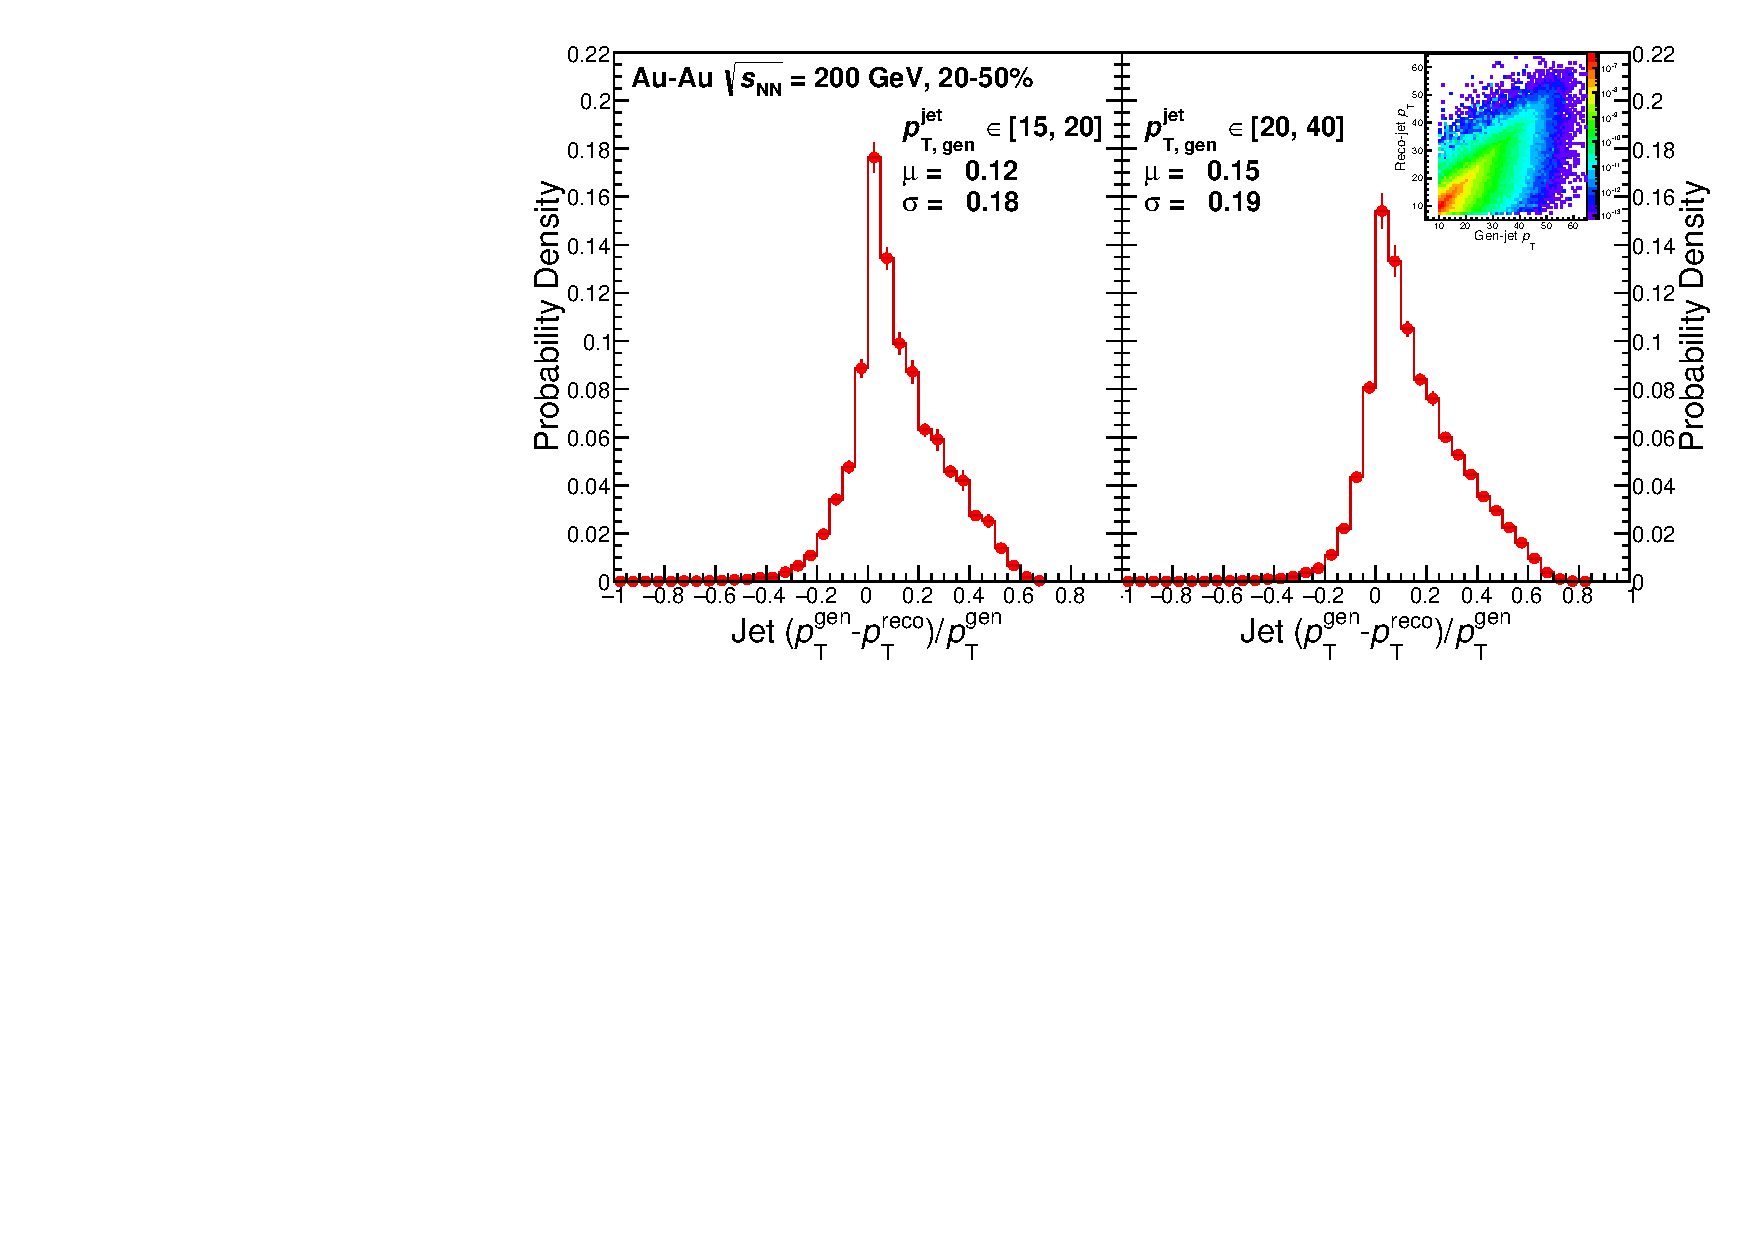
\includegraphics[width=0.99\linewidth]{figures/EmbPlot_pt_resolution_w_inset.pdf}
	\caption[Jet-\(p_\mathrm{T}\) resolution and response matrix of the Au+Au embedding]{\Pt{jet} resolution for $15 < \ptGenJet < 20$ \GeVc (left) and $20 < \ptGenJet < 40$ \GeVc (right) $R=0.4$ full jets with the corresponding response matrix as an inset on the top right.  Jets are measured from all angles relative to the event plane in the 20--50\% most central events.  This comparison is for matched GEN-level to RECO-level jets. }
	\label{fig:jetptresWinset}
\end{figure}

The same embedding sample is used for a closure test of the analysis chain.
%
The associated yields and jet-peak widths are extracted from the RECO-level jets with the full analysis procedure, including the mixed-event correction taken from data and the RPF background subtraction, and compared to those of the matched GEN-level jets, whose correlations with the final-state PYTHIA\mbox{-}6 particles contain no combinatorial background.
%
The comparison is complicated by the tracking efficiency near a jet, which differs from the average efficiency used in the correction: above 2~\GeVc it is slightly lower inside \pttrigrange{15}{20} jets and slightly higher inside \pttrigrange{20}{40} jets than for an average track in the event.
%
After correcting the RECO-level near-side yields for this difference, the RECO/GEN ratio of the yields for \pttrigrange{20}{40} jets, shown in Fig.~\ref{fig:ClosureJ2040}, is consistent with unity on the away side.
%
The remaining deviations, on the near side in the highest \Pt{assoc} bin and in the lowest \Pt{assoc} bins for \pttrigrange{15}{20} jets, were traced to the limited statistics of the low-$\hat{p}_\mathrm{T}$ bins of the embedding, which enter with large weights.

\begin{figure}[!htbp]
	\centering
	% white box covers the stale "points displaced for visibility" label (single series only)
	\begin{tikzpicture}
		\node[anchor=south west, inner sep=0] (img) {\includegraphics[width=0.99\linewidth]{JHC/NearAwaySideYieldRatioRECO-GEN_J20-40_C20-50_onlyALL_withEffCorr.pdf}};
		\begin{scope}[x={(img.south east)}, y={(img.north west)}]
			\fill[white] (0.198,0.182) rectangle (0.420,0.228);
		\end{scope}
	\end{tikzpicture}
	\caption[Embedding closure test of the associated yields for 20--40~GeV/\(c\) jets]{Embedding closure test: ratio of the near-side (left) and away-side (right) associated yields extracted from RECO-level jets to those of the matched GEN-level jets vs \Pt{assoc}, for \pttrigrange{20}{40} full jets embedded in 20--50\% central \AuAu events, all orientations relative to the event plane combined. The RECO-level near-side yields are corrected for the tracking efficiency inside jets (see text). The gray bands are the uncertainties of the RPF background fit.}
	\label{fig:ClosureJ2040}
\end{figure}

\subsection{Systematic uncertainties} \label{sect:SysUnc}
The systematic uncertainties fall into three classes that differ in how they are correlated, and therefore in how they are shown on the results.
%
(i) Sources that change the overall normalization of the correlation functions, independently of \dphi and of the jet orientation, are combined into a global scale uncertainty: the single-track reconstruction efficiency, the normalization of the mixed events, and the event-plane resolution.
%
(ii) Sources that change the level of the correlation functions in a way that depends on \Pt{assoc} and on the jet orientation are shown as colored scale bands: the shape of the pair acceptance in \deta and the jet-energy-shift (JES) correction.
%
(iii) The uncertainty of the RPF background fit, obtained from the covariance matrix of the fit, varies from point to point in \dphi and is correlated between points and between orientations; it is shown as a gray band.
%
Each source is described below.

The 5\% uncertainty on the single-track reconstruction efficiency (Sec.~\ref{sec:TrackTowerSel}) directly scales the number of associated hadrons, and hence the yields, while leaving the shape of the correlation functions unchanged.
%
The mixed-event normalization uncertainty is the uncertainty of the constant fitted to the plateau of the pair acceptance (Sec.~\ref{sect:MixedEventsUnc}).
%
The event-plane resolution enters only through the background parametrization, since the signal itself is not corrected for the resolution (Sec.~\ref{sec:EPReco}); varying it by $\pm 1\%$ changes the results negligibly.

The systematic uncertainties are summarized in Tabs.~\ref{Tab:SystematicSummary}, \ref{Tab:SystematicSummaryEPdep}, and~\ref{Tab:SystematicSummaryEPdep2040}.  Tab.~\ref{Tab:SystematicSummary} lists the sources of systematic uncertainties which are independent of the angle relative to the event plane.  These sources include the single-track reconstruction efficiency (Sec.~\ref{sec:TrackTowerSel}), 
%contamination from secondaries (Sec.~\ref{sect:STARdet}), 
uncertainties in the mixed events due to their normalization and shape in \dphi (Sec.~\ref{sect:MixedEventsUnc}), and uncertainties in the event-plane resolution (Sec.~\ref{sect:Method}).  The uncertainties are added in quadrature and lead to a 6\% uncertainty in the scale of the correlation functions and yields with the single-track reconstruction efficiency being the dominant source.  This uncertainty is uncorrelated for different associated-particle momenta.

\begin{table}[!htbp]
	\caption[Systematic uncertainties independent of the jet orientation]{Summary of systematic uncertainties which are independent of the angle relative to the event plane and the momentum for both \pttrigrange{15}{20} and \pttrigrange{20}{40} in 20--50\% central \AuAu collisions.}
	\label{Tab:SystematicSummary}
	\centering % used for centering table
	\begin{tabular}{l | c} % centered columns
		\hline % inserts double horizontal lines
		Source & Uncertainty \% \Tstrut \Bstrut \\ % inserts table heading
		\hline % inserts single horizontal line
		Single particle reconstruction efficiency & 5 \\
		%\hline
		%Contamination & 1 \\
		\hline
		Mixed event (shape \dphi) & negligible \\
		\hline
		Mixed event normalization & $< 1.25$ \\ 
		\hline
		Event-plane resolution &  $< 1$ \\ 
		\hline
	\end{tabular}
\end{table}

Additional uncertainties, highly dependent on the angle of the jet relative to the event plane and the associated particles' momentum, are summarized in Tabs.~\ref{Tab:SystematicSummaryEPdep} and~\ref{Tab:SystematicSummaryEPdep2040}.  These include the impact of the scale uncertainty from the acceptance shape (Sec.~\ref{sect:MixedEvents}, Eq.~\ref{Eqtn:alpha}) and the RPF background fit (Sec.~\ref{sect:CorrBkgd}) on the associated yield and jet-peak width results.  These uncertainties are compared for two associated particle momentum bins (1.0--1.5 and 3.0--4.0~\GeVc) to highlight how much of an impact the background has at low momenta.  The uncertainty arising from the RPF background subtraction is non-trivially correlated point-to-point in \dphi and for different orientations of the jet relative to the event plane, but is uncorrelated between different \Pt{assoc} bins.  The acceptance-correction uncertainty on the shape in \deta is also correlated for different orientations of the jet relative to the event plane and uncorrelated across \Pt{assoc} bins.  The acceptance-shape uncertainty is the dominant source at low momenta, while being more comparable to the background uncertainty at larger momenta.  

Since no underlying-event subtraction is applied to the jets (Sec.~\ref{sec:JetRecoAuAu}), background particles that fall into the jet cone shift the reconstructed jet momentum upward, and the shift is larger for in-plane than for out-of-plane jets because the flow-modulated background is larger in-plane.
%
Jets in the different orientations therefore sample slightly different parton momenta for the same reconstructed \Pt{jet} class.
%
To account for this jet-energy shift (JES) and to provide an adequate comparison for the jet samples from different orientations relative to the event plane, a random-cone study was performed on the minimum-bias data of matching centrality selection: cones of radius 0.4 are placed at random positions within the jet acceptance, and the transverse momenta of the charged particles inside them are summed, in bins of the cone orientation relative to the event plane.
%
The mean summed momenta are found to be 0.388 \GeVc (in-plane), 0.344 \GeVc (mid-plane), and 0.308 \GeVc (out-of-plane), with a corresponding RMS of 0.4 \GeVc.
%
To determine the effect on the results, the correlation functions are also constructed for jet-momentum classes shifted by a fixed amount, and the resulting changes of the yields and widths are rescaled to the shifts found with the random cones.
%
The nominal yields and widths are corrected by these rescaled shifts, and the corresponding rescaled RMS is assigned as the JES uncertainty, which is added in quadrature to the acceptance-shape scale uncertainty.

% jet energy scale correction

%Both of these sources are stronger on the near-side at low-momenta, while being stronger on the away-side for higher momenta.

% ------------------------ 15-20 GeV ---------------------------------
\begin{table}[!htbp]
	%\begin{table}[H]
	\caption[Orientation-dependent systematic uncertainties for 15--20~GeV/\(c\) jets]{Summary of systematic uncertainties on the associated yields and widths calculated from the correlation functions due to the shape uncertainty coming from the shape of the acceptance correction in \deta, the correlated background-fit uncertainty, and the uncertainty associated with the jet energy shift (JES) correction, each varying with event-plane orientation bins.  They are displayed for \pttrigrange{15}{20} in 20--50\% central \AuAu collisions for \ptassocrange{1.0}{1.5} and \ptassocrange{3.0}{4.0} bins.  The values are expressed as a percent of the nominal value.}
	\label{Tab:SystematicSummaryEPdep}
	\centering
	\small
	\setlength{\tabcolsep}{4pt}
	\begin{tabular}{c | c | c | c | c | c | c}\hline
		\multirow{3}{*}{Source} & \multirow{3}{*}{Result} & \multirow{3}{*}{Orientation} & \multicolumn{4}{c}{Uncertainty \%} \\ \cline{4-7}
		&   &      & \multicolumn{2}{c|}{Near-side: \Pt{assoc} (\GeVc)} & \multicolumn{2}{c}{Away-side: \Pt{assoc} (\GeVc)} \Bstrut \\ \cline{4-7}     
		&   &      & 1.0--1.5 & 3.0--4.0 & 1.0--1.5 & 3.0--4.0 \\ \hline       
		
		\multirow{6}{*}{} & \multirow{3}{*}{Yield} & in-plane & 14 & 1.2 & 8.1 & 3.0  \\ \cline{3-7}
		& & mid-plane & 11 & 1.2 & 7.6 & 3.3 \\ \cline{3-7}
		Acceptance & & out-of-plane & 11 & 1.1 & 7.3 & 3.0 \\ \cline{2-7}
		shape & \multirow{3}{*}{Width} & in-plane & 5.2 & 0.6 & 4.3 & 2.4 \\ \cline{3-7}
		& & mid-plane    & 5.4 & 0.5 & 3.9 & 2.2 \\ \cline{3-7}
		& & out-of-plane & 4.3 & 0.4 & 4.9 & 2.1 \\ \cline{3-7}
		\hline
		
		\multirow{6}{*}{} & \multirow{3}{*}{Yield} & in-plane & 11 & 0.8 & 6.1 & 2.1 \\ \cline{3-7}
		& & mid-plane & 7.7 & 0.9 & 5.2 & 2.5 \\ \cline{3-7}
		Background & & out-of-plane & 7.4 & 0.7 & 4.7 & 2.1  \\ \cline{2-7}
		fit & \multirow{3}{*}{Width} & in-plane & 10 & 0.1 & 8.2 & 0.4 \\ \cline{3-7}
		& & mid-plane    & 10 & 0.1 & 7.5 & 0.4 \\ \cline{3-7}
		& & out-of-plane & 8.2 & 0.1 & 9.3 & 0.4 \\ \cline{3-7}
		\hline
		
		\multirow{6}{*}{} & \multirow{3}{*}{Yield} & in-plane & 1.8 & 3.7 & 4.9 & 4.0  \\ \cline{3-7}
		& & mid-plane & 2.8 & 2.5 & 1.4 & 4.2 \\ \cline{3-7}
		JES & & out-of-plane & 3.7 & 3.3 & 4.8 & 4.2 \\ \cline{2-7}
		correction & \multirow{3}{*}{Width} & in-plane & 0.6 & 0.4 & 4.0 & $<$ 0.1 \\ \cline{3-7}
		& & mid-plane    & 0.2 & $<$ 0.1  & 7.9 & 1.5 \\ \cline{3-7}
		& & out-of-plane & 1.6 & 0.7 & 1.9 & 1.7 \\ \cline{3-7}
		
		\hline
	\end{tabular}
\end{table}

% ------------------------ 20-40 GeV ---------------------------------
\begin{table}[!htbp]
	%\begin{table}[!ht]
	%\begin{table}[H]
	\caption[Orientation-dependent systematic uncertainties for 20--40~GeV/\(c\) jets]{Summary of systematic uncertainties on the associated yields and widths calculated from the correlation functions due to the shape uncertainty coming from the shape of the acceptance correction in \deta, the correlated background-fit uncertainty, and the uncertainty associated with the JES correction, each varying with event-plane orientation bins.  They are displayed for \pttrigrange{20}{40} in 20--50\% central \AuAu collisions for \ptassocrange{1.0}{1.5} and \ptassocrange{3.0}{4.0} bins.  The values are expressed as a percent of the nominal value. }
	\label{Tab:SystematicSummaryEPdep2040}
	\centering
	\small
	\setlength{\tabcolsep}{4pt}
	\begin{tabular}{c | c | c | c | c | c | c}\hline
		\multirow{3}{*}{Source} & \multirow{3}{*}{Result} & \multirow{3}{*}{Orientation} & \multicolumn{4}{c}{Uncertainty \%} \\ \cline{4-7}
		&   &      & \multicolumn{2}{c|}{Near-side: \Pt{assoc} (\GeVc)} & \multicolumn{2}{c}{Away-side: \Pt{assoc} (\GeVc)} \Bstrut \\ \cline{4-7}     
		&   &      & 1.0--1.5 & 3.0--4.0 & 1.0--1.5 & 3.0--4.0 \\ \hline           
		
		\multirow{6}{*}{} & \multirow{3}{*}{Yield} & in-plane & 35 & 1.2 & 22 & 2.5  \\ \cline{3-7}
		& & mid-plane & 39 & 1.2 & 22 & 2.2 \\ \cline{3-7}
		Acceptance & & out-of-plane & 59 & 0.9 & 37 & 1.6 \\ \cline{2-7}
		shape & \multirow{3}{*}{Width} & in-plane & 30 & 0.7 & 8.4 & 1.9 \\ \cline{3-7}
		& & mid-plane    & 22 & 0.5 & 15  & 1.7 \\ \cline{3-7}
		& & out-of-plane & 19 & 0.4 & 28  & 1.2 \\ \cline{3-7}
		\hline
		
		\multirow{6}{*}{} & \multirow{3}{*}{Yield} & in-plane & 13 & 1.0 & 8.2 & 2.1 \\ \cline{3-7}
		& & mid-plane & 14 & 0.7 & 8.0 & 1.2 \\ \cline{3-7}
		Background & & out-of-plane & 22 & 0.9 & 14 & 1.5  \\ \cline{2-7}
		fit & \multirow{3}{*}{Width} & in-plane & 13 & 0.1 & 3.7 & 0.2 \\ \cline{3-7}
		& & mid-plane    & 10  & 0.1 & 6.8 & 0.2 \\ \cline{3-7}
		& & out-of-plane & 8.6 & $<$ 0.1 & 13  & 0.1 \\ \cline{3-7}
		\hline
		
		\multirow{6}{*}{} & \multirow{3}{*}{Yield} & in-plane & 0.2 & 0.4 & $<$ 0.1 & 2.6 \\ \cline{3-7}
		& & mid-plane & 1.1 & 0.3 & 2.1 & 2.9 \\ \cline{3-7}
		JES & & out-of-plane & 3.1 & 0.6 & 1.4 & 3.5  \\ \cline{2-7}
		correction & \multirow{3}{*}{Width} & in-plane & 1.2 & 0.5 & 3.3 & 0.3 \\ \cline{3-7}
		& & mid-plane    & 1.2 & 0.7 & 1.3 & 1.5 \\ \cline{3-7}
		& & out-of-plane & 2.2 & 0.1 & 0.2 & 1.9 \\ \cline{3-7} 
		\hline
	\end{tabular}
\end{table}

Tabs.~\ref{Tab:SystematicSummaryEPdep} and~\ref{Tab:SystematicSummaryEPdep2040} show the same pattern for both jet momentum classes.
%
The sources related to the background, the acceptance shape and the RPF fit, are largest at low \Pt{assoc} and fall steeply with it.
%
At \ptassocrange{1.0}{1.5} the jet signal is a small excess on top of a large combinatorial background, so a change of the level or shape of the pair acceptance, or of the fitted background, by a fraction of a percent of the background changes the subtracted signal by a large fraction of itself; at \ptassocrange{3.0}{4.0} the signal dominates and the same changes amount to about a percent.
%
The yields are more affected than the widths because a change of the background level shifts the whole pedestal under the jet peaks and therefore their integrals, while the widths respond only to changes of the shape near the peaks.
%
The JES uncertainty on the yields, by contrast, depends only weakly on \Pt{assoc}, staying at a few percent at both momenta, and it becomes the leading source at high \Pt{assoc}, where the background-related sources are small.

All the uncertainties are larger for the \pttrigrange{20}{40} jets, especially out-of-plane, and follow a less regular pattern than for the \pttrigrange{15}{20} jets; the JES correction, for example, affects the widths of the 20--40~\GeVc jets as much as their yields at low \Pt{assoc}.
%
The variations are evaluated on the data themselves, by re-binning the mixed events in \zvtx, refitting the background and repeating the analysis for shifted jet-momentum classes, and no Barlow check was applied to them.
%
They therefore include the statistical fluctuations of the varied analyses, which are larger for the smaller sample of \pttrigrange{20}{40} jets (Fig.~\ref{fig:NTrig}) and are the likely origin of the larger and irregular entries.

\section{Results} \label{sect:Results}
%\subsection{Yields}
\label{sect:Yields}
Charged particle yields associated with jets are found by integrating the background-subtracted correlation functions according to Eq.~\ref{Eqtn:Yield}.
%
The integration limits in \dphi for the near-side are $a=-\pi/3$ and $b=\pi/3$, while for the away-side, $a=2\pi/3$ and  $b=4\pi/3$.  The integration limits in \deta are the same for both the near-side and away-side, $c=-0.6$ and $d=0.6$.
%
The yield is computed as the difference of the integral of the measured signal+background distribution, which carries the statistical uncertainty, and the integral of the fitted background, whose uncertainty follows from Eq.~\ref{eqn:CovProp}; the two are reported separately.

Shown in Fig.~\ref{fig:AssocYields} are the near-side (left) and away-side (right) associated yields vs \Pt{assoc} for \pttrigrange{15}{20} (top) and \pttrigrange{20}{40} (bottom) full jets in 20--50\% centrality collisions.  The yields are compared for each orientation of the trigger jet reconstructed relative to the event plane (in/mid/out) for \Pt{assoc} $\in$ [1.0, 1.5], [1.5, 2.0], [2.0, 3.0], [3.0, 4.0], [4.0, 6.0], [6.0, 10.0] \GeVc.

The main feature is the steeply falling associated yield with increasing \Pt{assoc}, which occurs on both the near- and away-side.  Note that associated yields for \Pt{assoc} $\geq$ 2.0 \GeVc include jet constituents, which leads to the discontinuity at \Pt{assoc} = 2 \GeVc.  Additionally, the use of jets with `hard-cores' and containment of a tower associated to the firing event trigger can lead to a surface bias of the near-side jet.  This, however, maximizes the average path length the away-side recoil jets travel, increasing the likelihood of an interaction with the medium. An in-plane jet and an out-of-plane jet with the same \Pt{jet} would be expected to have different distributions of hard and soft constituents. An in-plane jet with less path traveled in the medium on average would be expected to show higher yields of constituents with higher \Pt{assoc} than the more quenched out-of-plane jet, which would be expected to show higher yields of constituents with lower \Pt{assoc}. While uncertainties are smaller for jets with \pttrigrange{15}{20}, both samples still lack any clear dependence on the event-plane angle.   This is an indication that modifications dependent on the average path length are smaller than the experimental uncertainties.  On the far right of the near- and away-side panels is the inclusive \Pt{assoc} bin with \ptassocrange{1.0}{10}. The associated yields of each event-plane orientation in the inclusive \Pt{assoc} selection are consistent with each other for the sample where \pttrigrange{15}{20}. However, in the jet sample with \pttrigrange{20}{40}, there are indications suggesting potential modifications. This potential modification is apparent on both the near- and away-side with the largest contributions coming from the lowest \Pt{assoc} bins.

% yield:
%\begin{figure}[!htbp]
\begin{figure}
	\begin{center}     
		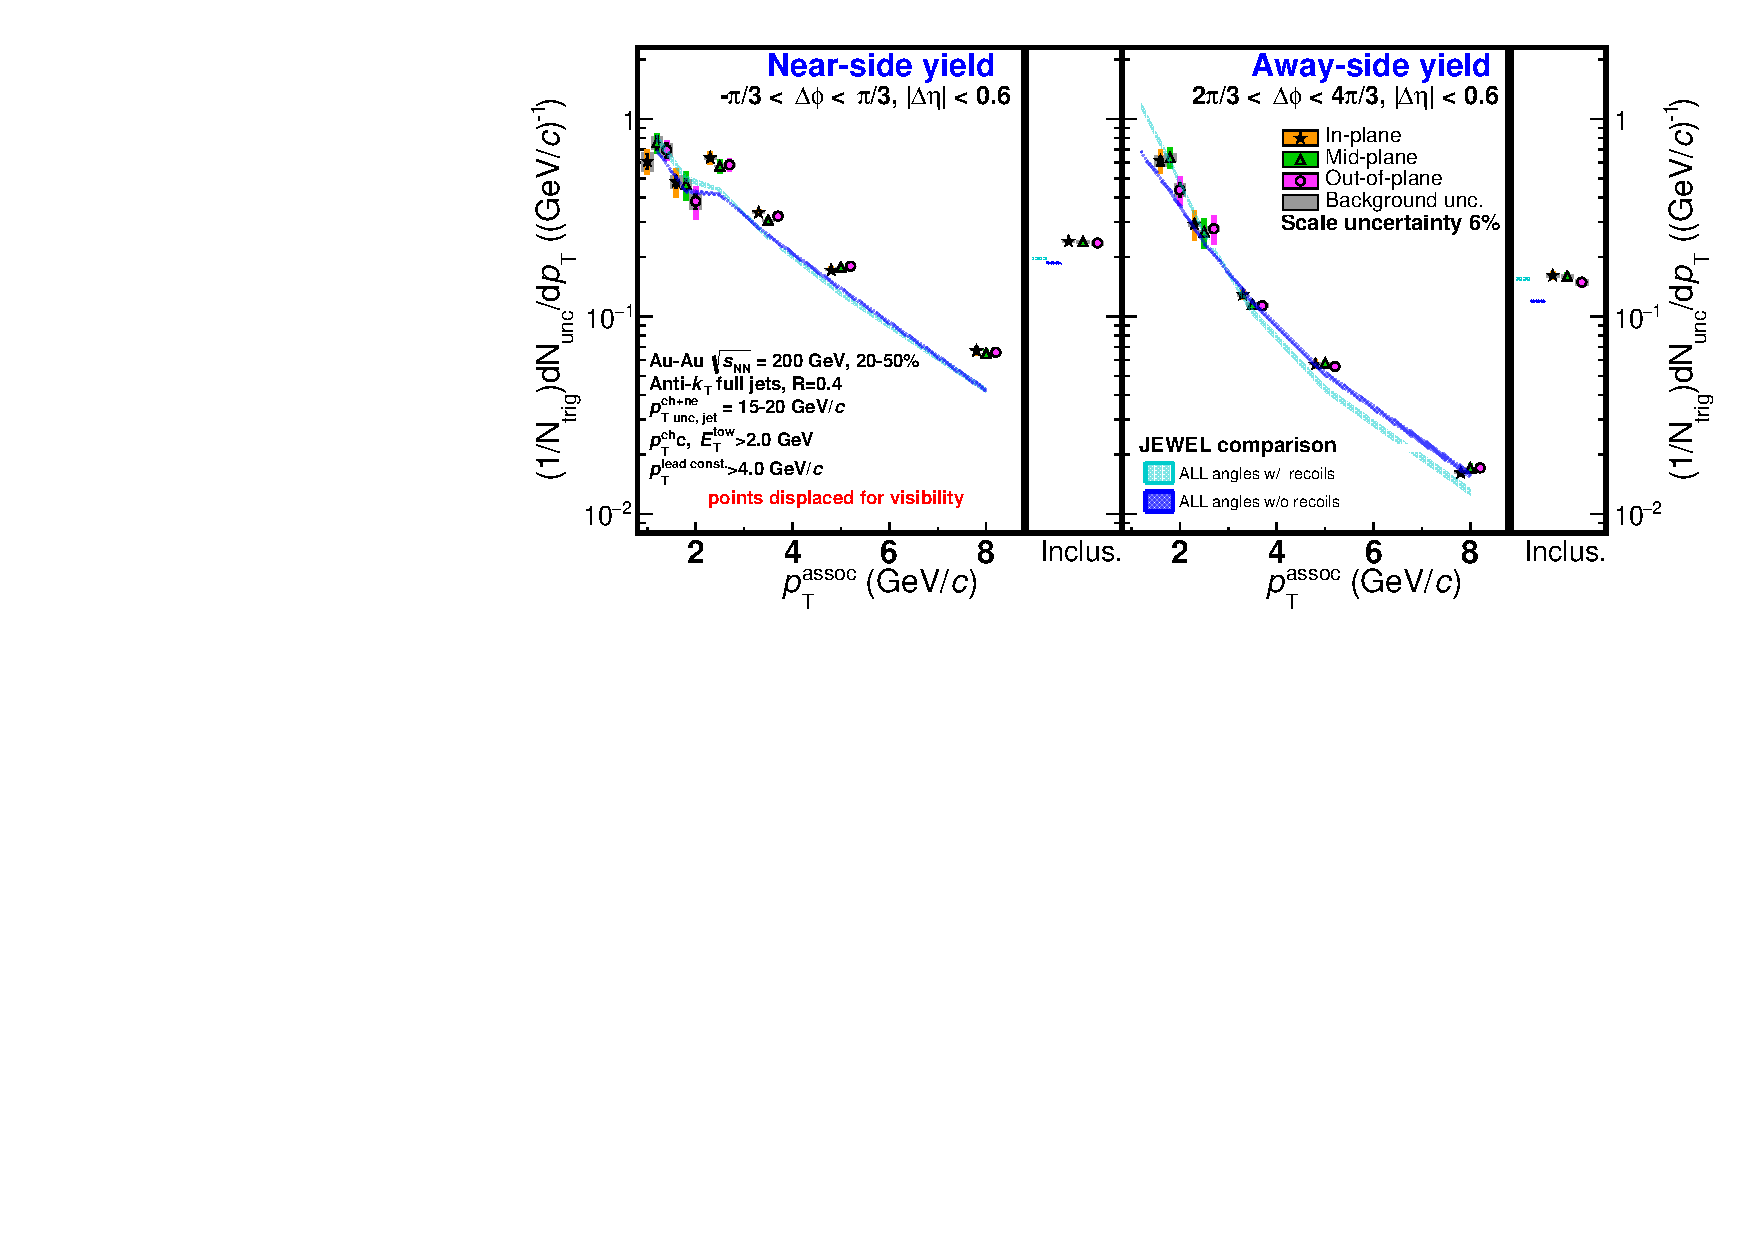
\includegraphics[width=\linewidth]{figures/JHC/results/NearAwaySideYield_J15-20_C20-50_wJEScorr_wJEWELerr.pdf}
		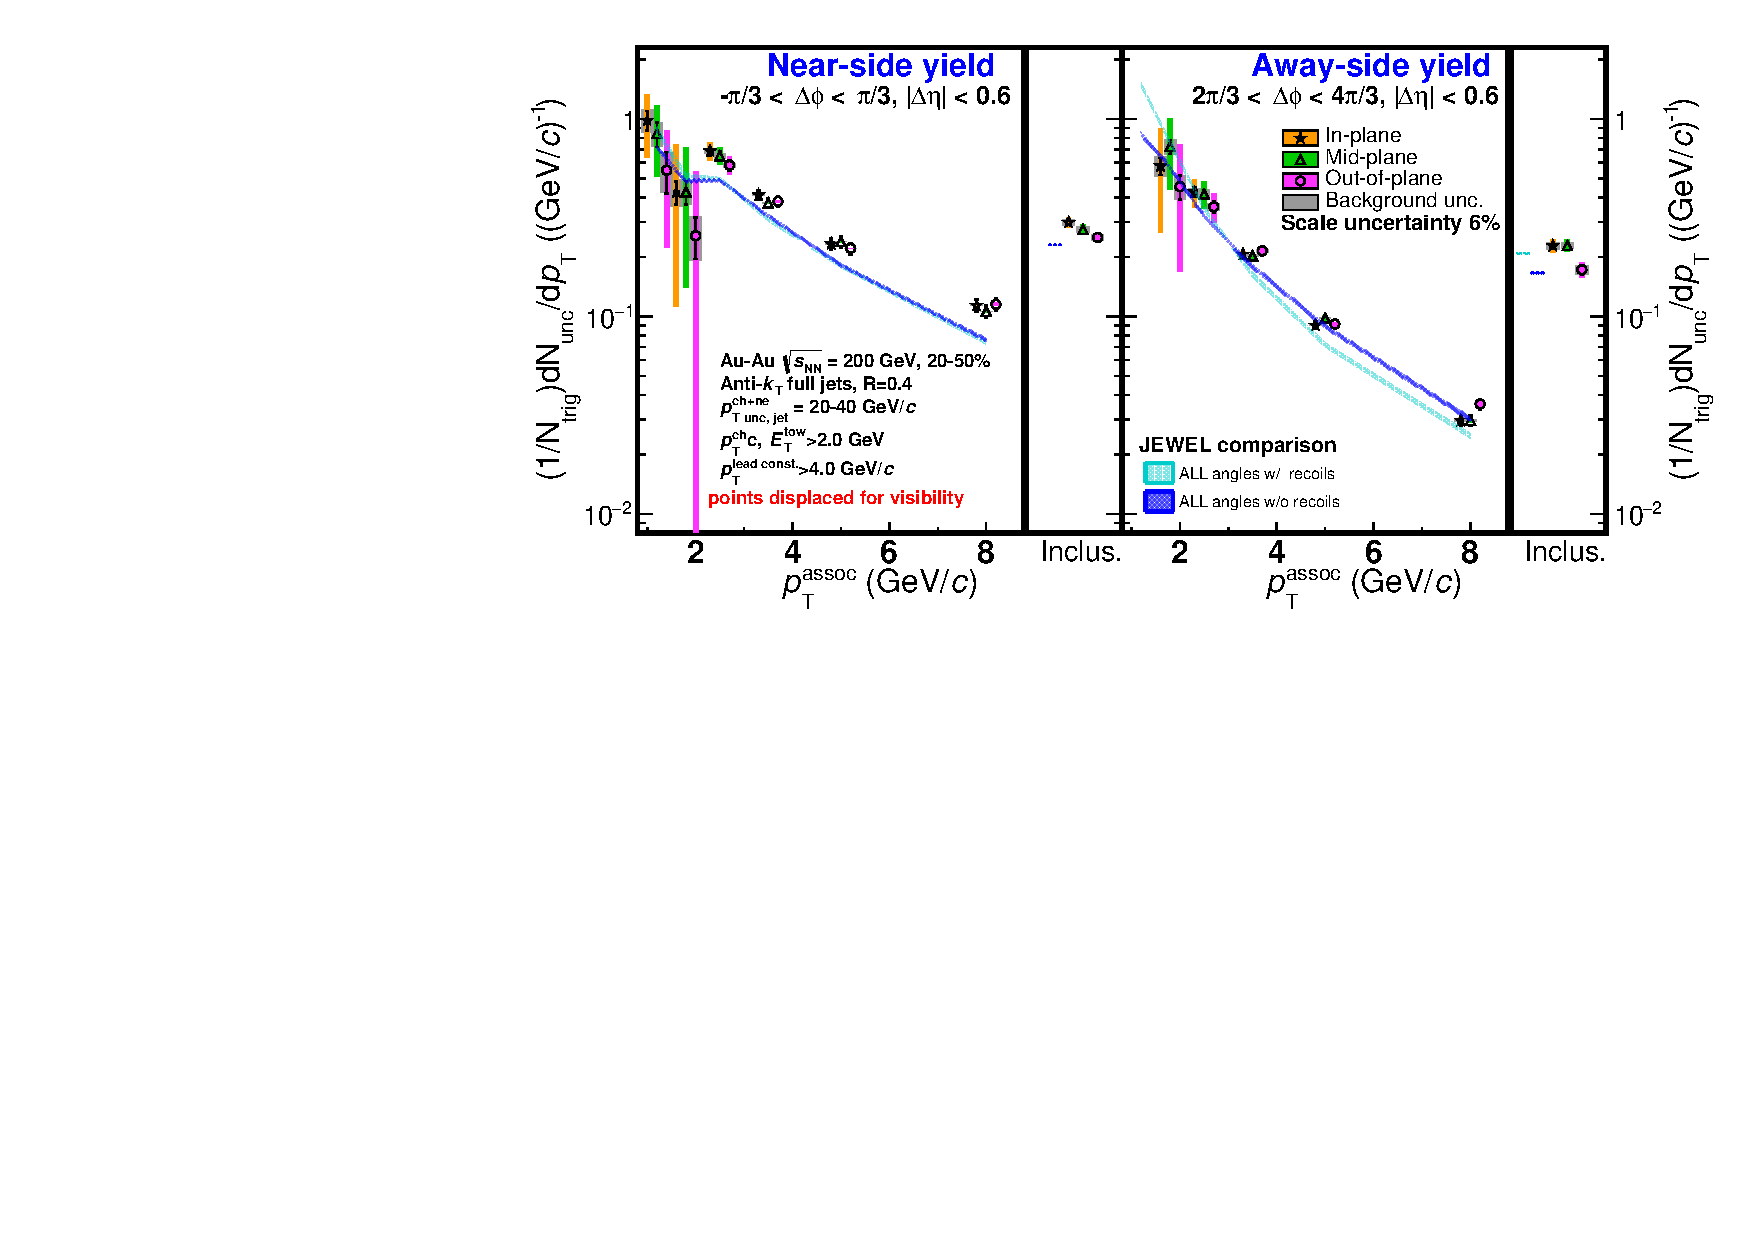
\includegraphics[width=\linewidth]{figures/JHC/results/NearAwaySideYield_J20-40_C20-50_wJEScorr_wJEWELerr.pdf}
		\caption[Near- and away-side associated yields as functions of \(p_\mathrm{T, assoc}\)]{Near-side (left) and away-side (right) uncorrected (unc.) associated yield vs \Pt{assoc} for 15--20 (top) and 20--40~\GeVc (bottom) full jets of 20--50\% centrality in \AuAu collisions.  The gray bands describe the systematic uncertainties of the background fits and are non-trivially correlated point-to-point.  The colored bands are scale uncertainties from the mixed-event acceptance shape and JES correction.  There is an additional 6\% global scale uncertainty.  Included on the far right of the near- and away-side panels is the inclusive transverse momentum bin from 1.0--10.0~\GeVc.  Points are displaced for visibility. } 
		\label{fig:AssocYields}
	\end{center}
\end{figure}

\label{sect:Widths}
The widths are calculated by fitting a Gaussian, $A\,\mathrm{e}^{-(\Delta\phi - \Delta\phi_0)^2/2\sigma^2}$, to the jet peak centered at $\dphi_0 = 0$ for the near-side and $\dphi_0 = \pi$ for the away-side.  The Gaussians are fitted separately, with a range of $|\Delta\phi|~<~\pi/3$ on the \ns and $|\Delta\phi - \pi|~<~\pi/3$ on the \as. The Gaussian fit is repeated with different values of the background parameters and the covariance matrix is used to propagate the uncertainties.  The scale uncertainties on the widths are given by $\sigma_{w}^{sc} = \frac{B}{\sigma_B} \times |\alpha - 1|$, where $\alpha$ (Eq.~\ref{Eqtn:alpha}) is the \Pt{assoc}-dependent scale factor associated with the acceptance shape when propagating the background determined in the $0.6 \leq |\deta| < 1.2$ to the region $|\deta| < 0.6$.  

Fig.~\ref{fig:JetWidths} shows that the jet peaks broaden with decreasing \Pt{assoc}.  This is expected from both collisional energy loss and gluon bremsstrahlung.  With out-of-plane jets expected to traverse a longer average path length than in-plane jets, this would lead to additional interactions with the medium and more subsequent re-scatterings resulting in a larger width for jets out-of-plane relative to in-plane.   Within the uncertainties there is no clear ordering.  This indicates the effect of path-length dependent energy loss is not large enough to be seen by the current precision of the data.  On the far right of the near- and away-side panels is the inclusive \Pt{assoc} bin with \ptassocrange{1.0}{10}.   The widths of each event-plane orientation in the inclusive selection for the sample with \pttrigrange{15}{20} are consistent.  Conversely, the \pttrigrange{20}{40} sample reveals indications of potential modifications.
This potential modification is apparent on both the near- and away-side and primarily comes from the lowest transverse momentum bins where sample size is the largest.

\begin{figure}
	\begin{center}     
		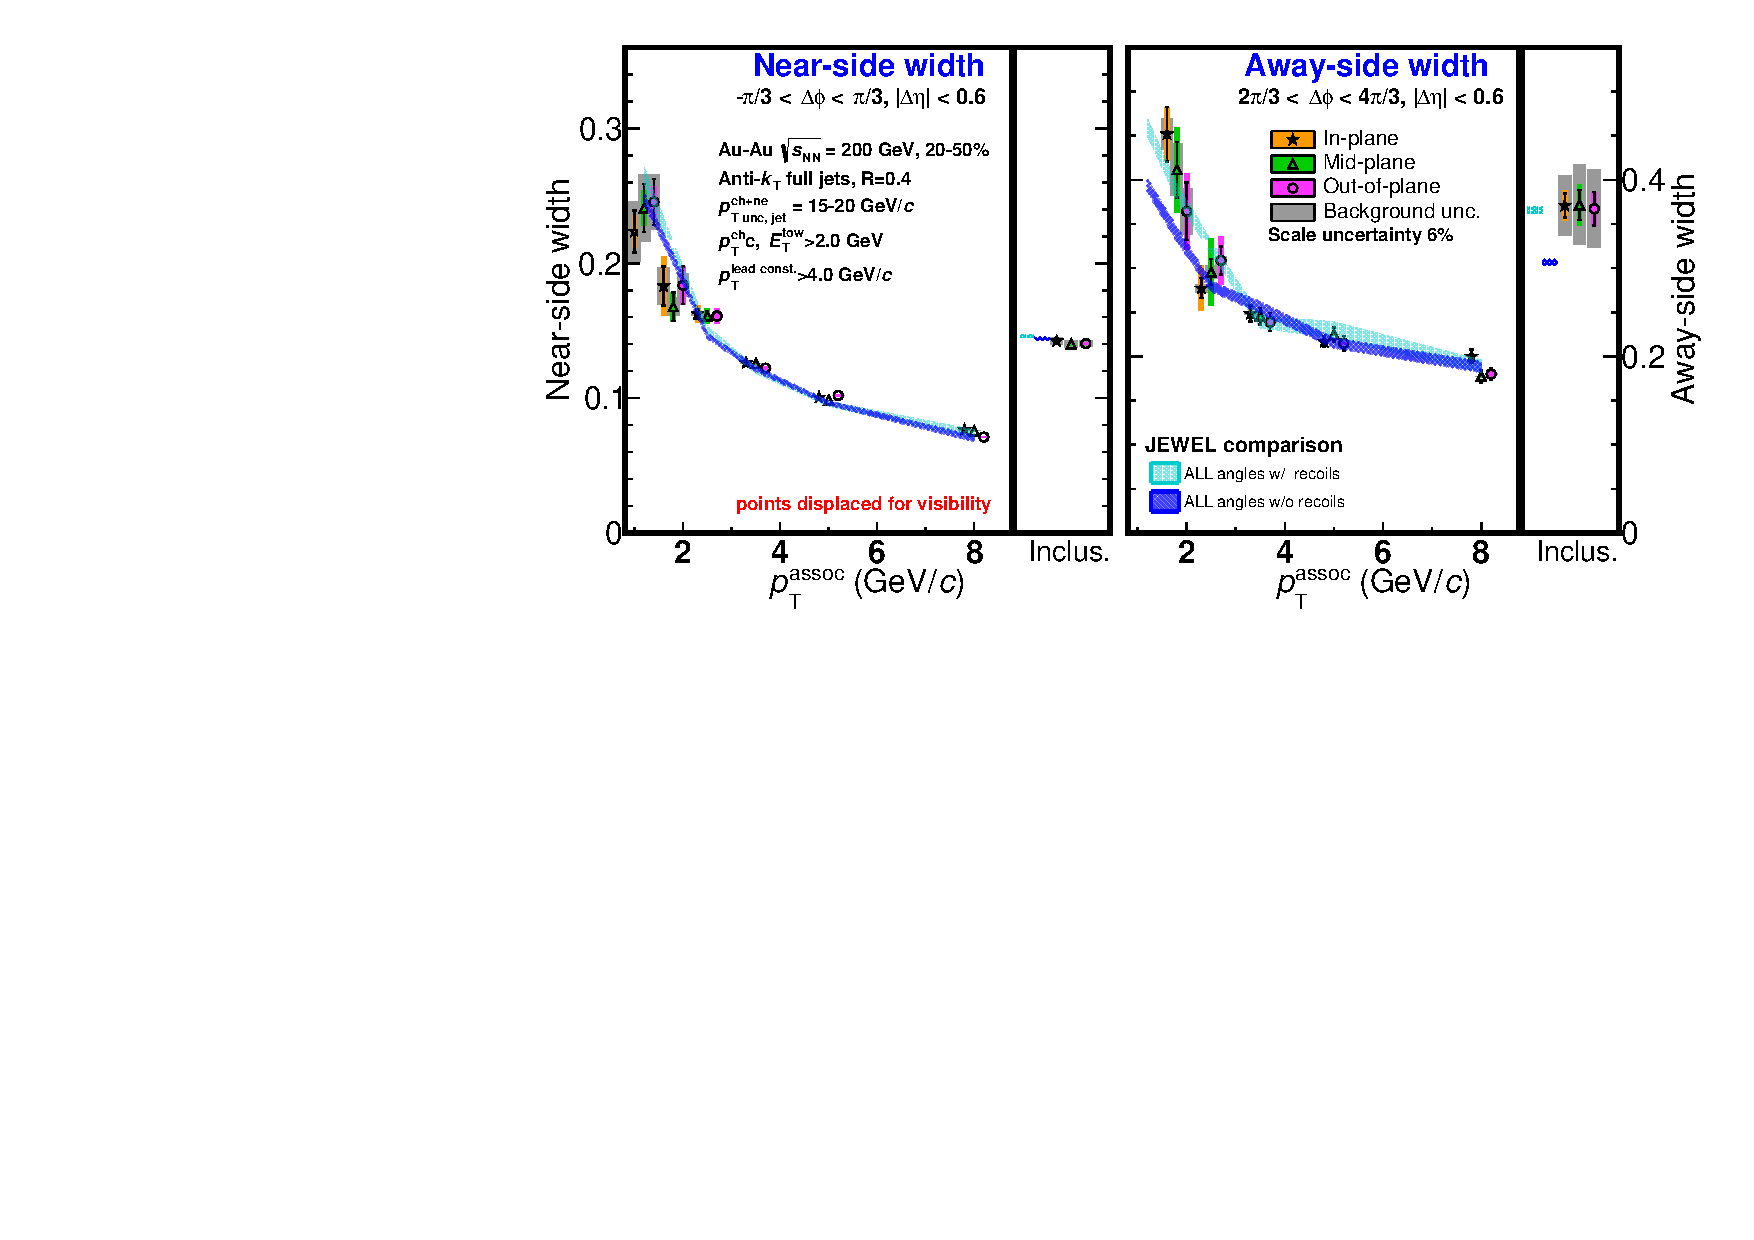
\includegraphics[width=\linewidth]{figures/JHC/results/NearAwaySideWidths_J15-20_C20-50_wJEScorr_wJEWELerr.pdf}
		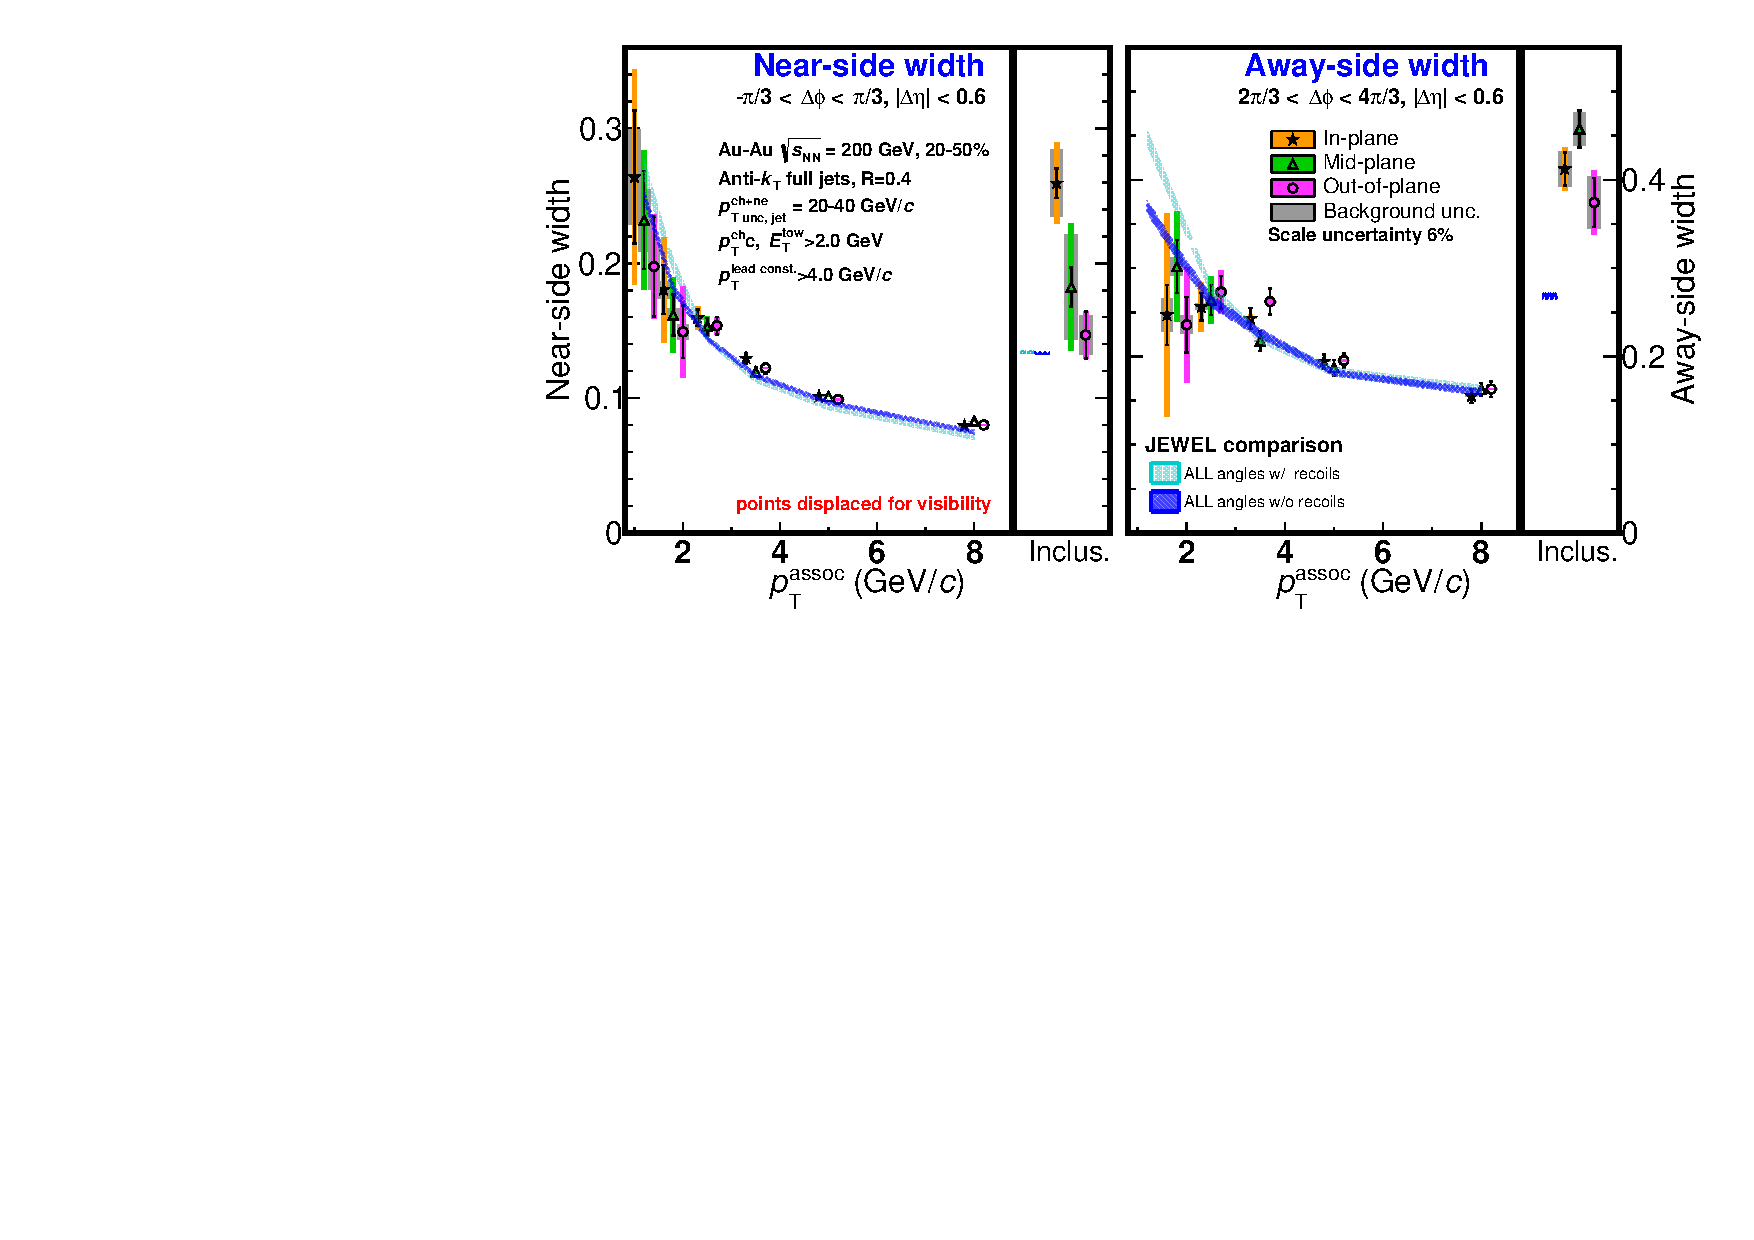
\includegraphics[width=\linewidth]{figures/JHC/results/NearAwaySideWidths_J20-40_C20-50_wJEScorr_wJEWELerr.pdf}
		\caption[Near- and away-side jet-peak widths as functions of \(p_\mathrm{T, assoc}\)]{Near-side (left) and away-side (right) jet width vs \Pt{assoc} for 15--20 (top) and 20--40~\GeVc (bottom) full jets of 20--50\% centrality in \AuAu collisions.  The widths are extracted from the Gaussian fit to the jet peak.  The gray bands describe the systematic uncertainties of the background fits which are non-trivially correlated point-to-point.  The colored bands are scale uncertainties from the mixed-event acceptance shape and JES correction.  There is an additional 6\% global scale uncertainty.  Included on the far right of the near- and away-side panels is an inclusive transverse momentum bin from 1.0--10.0~\GeVc.  Points are displaced for visibility. }
		\label{fig:JetWidths}
	\end{center}
\end{figure}

The measurements presented in Figs.~\ref{fig:AssocYields} and~\ref{fig:JetWidths} are compared to calculations from JEWEL introduced in Sec.~\ref{sec:eventGenerators}, with and without the recoil partons kept in the event. Without recoils, the momentum lost by the jet leaves the event, which models the energy loss of the hard part of the jet; with recoils, the momentum of the jet is conserved, but the recoils also add energy and particles to the dijet, and an experimental analysis likely measures some, but not all, of them, as they are often indistinguishable from the background.

Due to the dominant impact of jet-by-jet fluctuations on partonic energy loss over path-length dependence~\cite{Milhano:2015mng,Zapp:2013zya}, JEWEL only predicts a very slight event-plane dependence which is well below the systematic uncertainty in the measurement.  Variations among event-plane orientations were not seen at the 10\% level.  This is therefore consistent with path-length dependence having an insignificant impact compared to jet-by-jet fluctuations in energy loss.  Fluctuations in the density of the medium may also suppress observable path-length dependence and are not included in the JEWEL model.  However,  higher precision JEWEL calculations may be needed to discern any potential event-plane dependent effects.  The JEWEL comparisons are therefore shown for the sample integrated over all angles relative to the event plane and compared to the results from data, so that the event-plane resolution does not enter the comparison.  Comparisons show that the away-side is well described in terms of both the associated yields and widths by including recoils at low \Pt{assoc}, while at high \Pt{assoc}, the yields are better described by not including recoils and the widths have similar results to within uncertainties for both cases.  When looking at the near-side, the widths are quite similar at high \Pt{assoc} with slightly larger values when including recoils at low \Pt{assoc}.  For the associated yields at high \Pt{assoc}, both JEWEL cases are similar to each other, but underestimate the data and including recoils has larger yields that better match the data at low \Pt{assoc}.

\label{sect:YieldRatio}
To better quantify and examine the event-plane dependence of the yields, ratios were taken of mid-plane yields relative to in-plane yields and out-of-plane yields relative to in-plane yields.  The advantage of taking ratios is a reduction in systematic uncertainties due to cancellation of uncertainties from several sources.  The propagation of uncertainties follows Sec.~\ref{sect:RPF}.  The yield ratio is expressed as:

\begin{equation}
	r = \frac{Y_A}{Y_B} = \frac{Y_A^{\rm meas} - Y_A^{\rm bkgd}}{Y_B^{\rm meas} - Y_B^{\rm bkgd}},
	\label{eqn:YieldRatio}
\end{equation}

\noindent where A and B denote different event-plane orientations of the yield.  The statistical uncertainties, which come only from the completely uncorrelated terms $Y_A^{\rm meas}$ and $Y_B^{\rm meas}$, are calculated as: 

\begin{equation}
	\sigma^{\rm stat}_r = \left|\frac{1}{r}\right|\sqrt{\left(\frac{\sigma_A}{Y_A}\right)^2 + \left(\frac{\sigma_B}{Y_B}\right)^2}.
	\label{eqn:StatRatio}
\end{equation}

\noindent The scale uncertainties, displayed as colored bands on the yield and width plots, are correlated and completely cancel in the ratio.  Uncertainties from the RPF background subtraction are propagated with Eq.~\ref{eqn:CovProp}, but now applied to Eq.~\ref{eqn:YieldRatio}, which includes correlated background terms in the numerator and denominator of the ratio, so that part of the background uncertainty cancels.  The correlated background uncertainties are given by:

\begin{equation}
	\sigma^{\rm bkgd}_r = \sqrt{\sum_{i=0}^{N} \sum_{j=0}^{N} \frac{\partial r}{\partial p_i} \frac{\partial r}{\partial p_j} \sigma_{ij}}.
	\label{eqn:SysRatio}
\end{equation}

Where, $p_i$'s are the parameters of the RPF fits. Fig.~\ref{plot:YieldRatio_C20-50} shows the near-side (left) and away-side (right) associated-yield ratios of out-of-plane/in-plane and mid-plane/in-plane for 15--20 (top) and 20--40~GeV/\(c\) (bottom) jets.
%
The ratios are not corrected for the finite event-plane resolution (Sec.~\ref{sec:EPReco}): a real difference between the orientations would appear in them reduced to about half of its size.

For \pttrigrange{15}{20}, the out-of-plane to in-plane associated-yield ratio shows slight enhancement out-of-plane relative to in-plane at low \Pt{assoc}, although the effect is small.  This can potentially be due to additional induced gluon radiation that out-of-plane and mid-plane jets would experience relative to in-plane jets, possibly from the longer path length traversed by jets that are not in-plane.   Deviations of the yield ratios from 1.0 are not statistically significant on the away-side, although a small suppression is seen in-plane relative to both mid-plane and out-of-plane on both the near-side and the away-side for \ptassocrange{2.0}{5.0} for out/in.  The suppression is expected to occur at a higher momentum fraction ($z$) of the jet.  On the away-side, the effects are favoring a redistribution of energy from high-momentum constituents to lower momentum constituents.  
%However, the away-side measurement is not sensitive enough to the potential effects because the uncertainties associated with the result are dominated by both the statistics and the JES correction.
%the shift in energy to reconstructed jets from varying $v^{jet}_2$ between event-plane orientations.

For \pttrigrange{20}{40} the near-side ratios are consistent with 1.0 with some movement at the two lowest \Pt{assoc} bins.  On the away-side, mid/in is consistent with 1.0 with a little enhancement and out/in has an enhancement at high \Pt{assoc} and suppression at low \Pt{assoc}. This observation contradicts the expectations.  If in-plane jets interact less, the ratios are expected to be $< 1.0$ at high \Pt{assoc} and $> 1.0$ at low \Pt{assoc}.  This is a reminder of the competing effects in the analyzed momentum range, and it is an indication that the expected path-length effects due to jet energy loss are dominated by the fluctuations in the medium.

%\begin{figure}[!htbp]
\begin{figure}
	\begin{center}     
		\includegraphics[width=\linewidth]{JHC/results/YieldRatio_J15-20_C20-50_wJEScorr.pdf}
		\includegraphics[width=\linewidth]{JHC/results/YieldRatio_J20-40_C20-50_wJEScorr.pdf}
		\caption[Out-of-plane/in-plane and mid-plane/in-plane associated-yield ratios]{Near-side (left) and away-side (right) associated-yield ratios (of out-of-plane and mid-plane to in-plane) vs \Pt{assoc} for 15--20 (top) and 20--40 (bottom)~GeV/\(c\) full jets in 20--50\% centrality collisions.  The gray bands describe the systematic uncertainties of the background fits which are non-trivially correlated point-to-point.  The colored bands are scale uncertainties from the JES correction.  Points are displaced for visibility. }
		\label{plot:YieldRatio_C20-50}
	\end{center}
\end{figure}

Alternatively, the initial geometry within specific centrality bins may be fluctuating at a larger magnitude than any possible event-plane dependence~\cite{Noronha-Hostler-RAAv2,PhysRevLett.116.252301}.  The possibility of this occurrence can be studied by looking at the initial configuration and selecting low and high ellipticity events by  using the $q_n$ flow vector found within a selected centrality range.  Since the present measurement is already limited by statistics, such a selection, which keeps only a fraction of the events, would require the larger \AuAu datasets recorded by STAR in 2023 and 2025~\cite{RHICRunSummary}.

To study the impact of surface bias and event-plane resolution, a check was performed to investigate the systematic change in the ratio of yields (out/in, mid/in) with the angle of the event plane by fitting a constant to Fig.~\ref{plot:YieldRatio_C20-50} for jets with \pttrigrange{15}{20} (top) and \pttrigrange{20}{40} (bottom).  The systematic uncertainties are treated as uncorrelated point-to-point and added to the statistical uncertainties in quadrature.  The results are shown in Tabs.~\ref{Tab:RatioFits_J15-20} and~\ref{Tab:RatioFits_J20-40} and are consistent with one.  Care should be taken when interpreting the results, as various effects can be in play and medium modifications could give way to a \Pt{assoc} dependence. This \Pt{assoc} dependence can be seen as an enhancement of associated yields for $\Pt{assoc} \geq$ 2 \GeVc on the near-side from the geometric kinematic biases due to the ``hard-core'' requirement of jet reconstruction.   

%======================================================================
\begin{table}
	%\begin{table}[!ht]
	\caption[Constant fits to the associated-yield ratios for 15--20~GeV/\(c\) jets]{Results of fits to Fig.~\ref{plot:YieldRatio_C20-50} (top panel: 15--20~\GeVc jets) to a constant $c$, the $\chi^2$ over the number of degrees of freedom (NDF), the number of standard deviations $\sigma$ of $c$ from one, and the range of $c$ within a 90\% confidence limit (CL).}
	\label{Tab:RatioFits_J15-20}
	\centering % used for centering table
	\begin{tabular}{c | c c | c c} % entered columns (5 columns)
		\hline
		& \multicolumn{2}{c |}{Near-side}  & \multicolumn{2}{c}{Away-side}  \\
		parameter & $Y_{\mathrm{out}} / Y_{\mathrm{in}}$  & $Y_{\mathrm{mid}} / Y_{\mathrm{in}}$   & $Y_{\mathrm{out}} / Y_{\mathrm{in}}$  & $Y_{\mathrm{mid}} / Y_{\mathrm{in}}$  \\ \hline
		%XXX OLD
		%$c$ &  0.977 $\pm$  0.026 &  0.999 $\pm$  0.029 &  0.885 $\pm$  0.028 &  0.965 $\pm$  0.032 \\
		%$\chi^2$/NDF &  1.8  & 0.41  & 0.98 & 0.63 \\
		%$\sigma$ & -0.9 & -0.0 & -4.1 & -1.1 \\
		%90\% CL & 0.91 -- 1.05 & 0.96 -- 1.04 & 0.83 -- 0.94 & 0.91 -- 1.02 \\
		% ---- before JES Shift correction ----
		%$c$          & 0.949 $\pm$ 0.02 & 0.983 $\pm$ 0.019 & 0.914 $\pm$ 0.023 & 0.979 $\pm$ 0.022 \\
		%$\chi^2$/NDF & 3.4              & 0.35              & 3                 & 0.39 \\
		%$\sigma$     & -2.6             & -0.9              & -3.7              & -1.0 \\
		%90\% CL      & 0.88 -- 1.02     & 0.96 -- 1.01      & 0.83 -- 0.99      & 0.95 -- 1.01 \\
		$c$          & 0.93 $\pm$ 0.042 & 0.949 $\pm$ 0.038 & 0.89 $\pm$ 0.065 & 0.997 $\pm$ 0.066 \\
		$\chi^2$/NDF & 0.68             & 0.67              & 0.71             & 0.18 \\
		$\sigma$     & -1.6             & -1.3              & -1.7             & -0.1 \\
		90\% CL      & 0.86 -- 1.00     & 0.89 -- 1.01      & 0.78 -- 1.00     & 0.94 -- 1.05 \\
		\hline
	\end{tabular}
\end{table}

%======================================================================
% === Comment out table for 20-40 GeV jets, ====
\begin{table}
	%\begin{table}[!ht]
	\caption[Constant fits to the associated-yield ratios for 20--40~GeV/\(c\) jets]{Results of fits to Fig.~\ref{plot:YieldRatio_C20-50} (bottom panel: 20--40~\GeVc jets) to a constant $c$, the $\chi^2$ over the number of degrees of freedom (NDF), the number of standard deviations $\sigma$ of $c$ from one, and the range of $c$ within a 90\% confidence limit (CL).}
	\label{Tab:RatioFits_J20-40}
	\centering % used for centering table
	\begin{tabular}{c | c c | c c} % entered columns (5 columns)
		\hline
		& \multicolumn{2}{c |}{Near-side}  & \multicolumn{2}{c}{Away-side}  \\
		parameter & $Y_{\mathrm{out}} / Y_{\mathrm{in}}$  & $Y_{\mathrm{mid}} / Y_{\mathrm{in}}$   & $Y_{\mathrm{out}} / Y_{\mathrm{in}}$  & $Y_{\mathrm{mid}} / Y_{\mathrm{in}}$  \\ \hline
		%XXX OLD
		% $c$ &  0.921 $\pm$  0.042 &  0.998 $\pm$  0.053 &   1.06 $\pm$  0.047 &    1.1 $\pm$   0.05 \\
		% $\chi^2$/NDF & 0.36  & 0.73  &  3.9 & 0.43 \\
		% $\sigma$ & -1.9 & -0.0 & 1.2 & 2.0 \\
		% 90\% CL & 0.87 -- 0.97 & 0.91 -- 1.09 & 0.87 -- 1.24 & 1.03 -- 1.17 \\
		% --- before JES Shift correction ---
		%$c$          & 0.898 $\pm$ 0.032 & 0.969 $\pm$ 0.033 & 0.989 $\pm$ 0.035 & 1.04 $\pm$ 0.033 \\
		%$\chi^2$/NDF & 0.84              & 0.44              & 3.6               & 1.5 \\
		%$\sigma$     & -3.2              & -1.0              & -0.3              & 1.3 \\
		%90\% CL      & 0.84 -- 0.96      & 0.93 -- 1.01      & 0.86 -- 1.12      & 0.96 -- 1.13 \\
		$c$          & 0.874 $\pm$ 0.043 & 0.937 $\pm$ 0.043 & 0.752 $\pm$ 0.064 & 1.02 $\pm$ 0.075 \\
		$\chi^2$/NDF & 1.4               & 0.19              & 2.1               & 0.49 \\
		$\sigma$     & -2.9              & -1.5              & -3.9              & 0.2 \\
		90\% CL      & 0.77 -- 0.98      & 0.90 -- 0.97      & 0.56 -- 0.94      & 0.91 -- 1.12 \\
		\hline
	\end{tabular}
\end{table}

\section{Conclusions} \label{sect:Summary}
The measurement of jet-hadron correlations relative to the event plane is reported for the 20--50\% most central events in \AuAu collisions at \sNN{200}{GeV} in STAR. 
%
Partonic interactions are directly related to the distance traversed in the medium, so it is expected that medium-induced jet modifications should depend on the path length. 
%
The angle of the jet, measured with respect to the event plane, is correlated on average with the jet's path length through the medium. 
%
In this analysis, the average path length of away-side jets is potentially increased due to the surface bias of the near-side trigger jet. 
%
This work utilizes the RPF background-subtraction method to remove the event-plane dependent background while reducing uncertainties and assumptions associated with previous background-subtraction techniques. 
%
Associated yields, their ratios, and jet-peak widths are extracted for each event-plane orientation and compared with different average path lengths and JEWEL model calculations. 
%
JEWEL performs better in describing the associated yields and widths at higher \Pt{assoc} when recoil partons are not included. 
%
Conversely, including recoil partons leads to JEWEL providing a better description of the lower \Pt{assoc} region. 
%
This study highlights the importance of conducting further tuning of Monte Carlo simulations to accurately describe the results in this analysis for jets that are biased towards hard-fragmented jets due to the HT-trigger and hard-core constituent requirements.

Within the precision of the current measurement at \sNN{200}{GeV}, the associated yields and jet-peak widths show no dependence on the event plane. 
%
The ratios derived from the associated yields are used to quantify the differences, but they do not deviate significantly from 1.0. For the \pttrigrange{20}{40} jets, there were indications of potential modifications observed in the inclusive bin of \ptassocrange{1.0}{10}.
%
The results presented in this study align with the findings observed in hadron-hadron and jet-hadron correlations reported in Ref.~\cite{Nattrass:2016cln} for RHIC and  Ref.~\cite{PhysRevC.101.064901} for LHC energies.  
%
The lack of clear event-plane dependence in the data indicates that any dependence of these modifications on the average path-length is less than the experimental uncertainties.